\pdfoutput=1
\documentclass[11pt]{amsart}
\usepackage{amsmath,amssymb,amsthm}
\usepackage[margin=1.2in]{geometry}
\usepackage{booktabs,adjustbox,xcolor,graphicx}
\usepackage[colorlinks=true,linkcolor=blue,citecolor=blue,urlcolor=blue]{hyperref}
\hypersetup{pdfauthor={Bernd Johannes Wuebben},
pdftitle={Hermitian--Yang--Mills flow and gluing on degenerating curves}}
\setlength{\emergencystretch}{2em}
\newtheorem{theorem}{Theorem}[section]
\newtheorem{proposition}[theorem]{Proposition}
\newtheorem{lemma}[theorem]{Lemma}
\newtheorem{corollary}[theorem]{Corollary}
\theoremstyle{definition}
\newtheorem{definition}[theorem]{Definition}
\newtheorem{example}[theorem]{Example}
\newtheorem{question}[theorem]{Question}
\theoremstyle{remark}
\newtheorem{remark}[theorem]{Remark}
\newcommand{\RR}{\mathbb R}
\newcommand{\CC}{\mathbb C}
\newcommand{\PP}{\mathbb P}
\newcommand{\cC}{\mathcal C}
\newcommand{\cP}{\mathcal P}
\newcommand{\cV}{\mathcal V}
\newcommand{\Herm}{\operatorname{Herm}}
\newcommand{\tr}{\operatorname{tr}}
\newcommand{\Ad}{\operatorname{Ad}}
\newcommand{\End}{\operatorname{End}}
\newcommand{\Geo}{\operatorname{Geo}}
\newcommand{\Log}{\operatorname{Log}}
\newcommand{\id}{\operatorname{id}}
\newcommand{\SU}{\operatorname{SU}}
\newcommand{\op}{\mathrm{op}}
\newcommand{\HS}{\mathrm{HS}}
\title[HYM flow and gluing]{Hermitian--Yang--Mills flow and gluing\\on degenerating curves}
\author{Bernd Johannes Wuebben}
\subjclass[2020]{53C07 (primary); 14D06, 58J35, 58J50 (secondary)}
\keywords{Hermitian--Yang--Mills flow, nodal degeneration, flat bundle,
small eigenvalue, gluing, matrix metric}
\date{November 11, 2026\\This version: November 11, 2026}

\begin{document}
% Private working manuscript; complete assembled reviews are pending.
\begin{abstract}
For a six-parameter degeneration of plane quartics, we approximate
Hermitian--Yang--Mills metric flow on flat unitary bundles with trivial
component connections and noncommuting gluing by a finite gradient
flow. Its energy is a sum of squared distances between positive
Hermitian matrices after unitary transport, weighted by neck capacities.
The integrated squared-distance comparison holds on time intervals
proportional to the shortest logarithmic neck length, uniformly in all
node-length ratios and as the gluing representation becomes reducible.
We prove relative asymptotics for every small linearized eigenvalue
and reach the comparison from an open class of bounded spatial initial
metrics with uniform component regularity after a negligible initial
layer. The comparison
holds for all time when the smallest effective eigenvalue times the
shortest logarithmic neck length stays bounded away from zero.
A second compact family permits independently vanishing component
holonomy and neck size. On the quartic family with equal node
parameters we determine the
leading Hodge metric on the unitary Schottky locus and asymptotically
recover projective gluing from low eigenvalues and component averages
of orthonormal eigensections in fixed unitary frames. On a finite class
of first-order rational-component smoothings, these observations and
the base-loop orientation determine unknown adjacency and the integral
symplectic conjugacy class of monodromy.
\end{abstract}
\maketitle
\section{Introduction}\label{sec:introduction}

When a compact Riemann surface develops nodes, a metric
on a bundle can equilibrate on the normalization components
long before the components equilibrate with one another.
The remaining variables are matrix metrics. Their coupling
depends on the fibre identifications at the nodes, including
cycle holonomy that cannot be removed by component frame
changes. We prove a finite nonlinear reduction of the
actual Hermitian--Yang--Mills metric flow in this setting.
The comparison allows independent node lengths and
noncommuting unitary gluing. It is accompanied by a complete
relative spectral theorem, entry from spatial initial
metrics, and geometric and inverse consequences.

The principal family smooths four projective lines in
general position. Its six nodes have independent exact
holomorphic equations $u_ev_e=\tau_e$; its smooth fibres
$C_\tau$ are plane quartics of genus three. We use the
metric induced by the Fubini--Study form, normalized so
that a line has area one. The construction in
Section~\ref{sec:geometry} gives a proper projective
family and, for every tuple $U=(U_e)\in\SU(r)^6$,
a holomorphic bundle with flat unitary connection $D_U$,
parallel metric $h_0$ and trivialized determinant.
Here $r\ge2$ is fixed. The component connections are
trivial, and fibre holonomy factors through the free
group of rank three of the dual graph $K_4$.
The bundles are polystable of degree zero and are
stable exactly when this representation is irreducible.

\subsection{The effective equation and the main theorem}
Transport $U_{ij}$ takes the $j$ component frame to the
$i$ frame. Set
\[
 L_e=\log(1/|\tau_e|),\qquad L_*=\min_eL_e,\qquad
 w_e=2\pi/L_e .
\]
All parameters are fixed during each flow, and the
degeneration limit is $L_*\to\infty$.
Let $A_i$ denote the limiting component areas, equal
to one for the chosen Fubini--Study metric. On the
real space of trace-free Hermitian tuples
$\cV=\bigoplus_{i=0}^3\Herm_0(r)$ define
\[
 M(X)=\sum_i A_i\tr(X_i^2),\qquad
 Q_{\tau,U}(X)=\sum_{e=ij}w_e
       \|X_i-U_{ij}X_jU_{ij}^*\|_{\HS}^2.
\]
Let $\nu_0\le\cdots\le\nu_{m-1}$ be the generalized
eigenvalues of $(Q_{\tau,U},M)$, including zeros,
where $m=4(r^2-1)$. The actual linearized operator is
$\Delta_{\tau,U}=D_U^*D_U$ on trace-free
$h_0$-Hermitian endomorphisms, with the unnormalized
area norm. Its eigenvalues are denoted by $\lambda_k$.

Write $\cP_r$ for the determinant-one positive
Hermitian matrices, with symmetric-space metric
$g_P(V,W)=\tr(P^{-1}VP^{-1}W)$ and distance $d$.
The finite potential and its negative gradient
equation, using the area-weighted product metric, are
\begin{equation}\label{eq:intro-finite}
 \begin{split}
 \Phi_{\tau,U}(\mathbf H)
   &=\frac12\sum_{e=ij}w_e
                d(H_i,U_{ij}H_jU_{ij}^*)^2,\\
 H_i^{-1}\dot H_i
   &=\frac1{A_i}\sum_{e=ij}w_e
                  \log(H_i^{-1}U_{ij}H_jU_{ij}^*).
 \end{split}
\end{equation}
The exact metric flow uses physical time $s$ and
the normalization $H^{-1}\partial_sH=-2i\Lambda F_H$.
For two metrics set
$\sigma(H,K)=\tr(H^{-1}K+K^{-1}H)-2r$.
It is intrinsic under frame changes and bounds
$d(H,K)^2$ from above.

We also specify an initial class that does not
require an already matched finite tuple. Put
$\rho=L_*^{-1}$, fix $0<\beta<1$ and $R_0>0$,
and write an initial metric as $h_0e^S$.
Let $\Omega_i(2\rho)\subset C_i$ be the complement
of the incidence discs of radius $2\rho$.
Pull $S$ back to these component exteriors using
the fixed geometric identifications and flat
frames of Section~\ref{sec:geometry}. Require
\begin{equation}\label{eq:intro-initial-class}
 \|S\|_{C^0(C_\tau)}
 +\inf_{\widetilde S_i|_{\Omega_i(2\rho)}=S_i}
           \sum_i\|\widetilde S_i\|_{C^{6,\beta}(C_i)}
 <R_0 ,
\end{equation}
where the extensions are trace-free Hermitian
matrices on the fixed components.
This is a nonempty open class on each smooth
fibre. Its radius is independent of the degeneration;
bounded smooth data on the middle necks may have
arbitrarily large derivatives.

A unitary frame identifies each endomorphism fibre
with $\operatorname{Mat}_r(\CC)$ and so specifies
the matrix-algebra marking used below.
Projective transport means the class of a unitary
edge map in $\operatorname{PSU}(r)=\SU(r)/Z(\SU(r))$.
After choosing a base vertex, cycle transports
are represented in its frame; changing that
frame conjugates all cycle maps simultaneously.

\begin{theorem}\label{thm:main}
The compact quartic family and flat bundles above
have the following properties.
\begin{enumerate}
\renewcommand{\labelenumi}{(\roman{enumi})}
\item There are $\gamma>0$ and $\epsilon(\tau)\to0$
as $L_*\to\infty$ such that
\[
 (1-\epsilon(\tau))\nu_k\le\lambda_k
 \le(1+\epsilon(\tau))\nu_k\quad(0\le k<m),
 \qquad \lambda_m\ge\gamma .
\]
The estimates are uniform in all node-length ratios
and all $U$. The kernel is naturally identified with the space of
tuples satisfying $X_i=\Ad(U_{ij})X_j$.

\item For finite initial tuples in a fixed bounded
ball, \eqref{eq:intro-finite} has a confined
all-time solution. It determines a smooth
determinant-one comparison metric $\widehat K(s)$
on the entire $C_\tau$, converging to $H_i(s)$
on fixed component compact subsets with error
$O(L_*^{-1})$. If the exact initial metric has
fixed positive bounds against $h_0$ and
$\eta=\int_{C_\tau}\sigma(H^{\mathrm{in}},\widehat K(0))\,dA_\tau$,
then, with $e_*=(1+\log L_*)^2/L_*$,
\[
 \sup_{0\le s\le TL_*}\int_{C_\tau}
       d(H(s),\widehat K(s))^2\,dA_\tau
       \le\eta+CTe_*\qquad(T\ge0).
\]
The constants are independent of $T$, the
node-length ratios and the unitary transports.

\item For the spatial initial class
\eqref{eq:intro-initial-class}, the component
flows select a bounded tuple $P$ and there is
a uniform preparation time $s_*\to\infty$,
$s_*/L_*\to0$, such that the comparison in
part~{\rm(ii)} applies to $H(s_*+s)$ and the
finite flow starting at $P$, with initial
error $\eta_*\to0$ uniformly over that class.

\item If $L_*\nu_0\ge\kappa>0$, then for the
initial data and discrepancy in part~{\rm(ii)}
\[
 \sup_{s\ge0}\int_{C_\tau}d(H(s),\widehat K(s))^2\,dA_\tau
 \le C\eta+C_\kappa e_*(1+|\log e_*|).
\]
The same conclusion holds after the preparation
in part~{\rm(iii)}, with $\eta_*$ in place of $\eta$.

\item On the common-node slice $\tau_e=t$, put
$L=\log(1/|t|)$. The graph representation
quotient $\SU(r)^{6,\mathrm{irr}}/\SU(r)^4$
embeds as a Lagrangian locus in the irreducible
flat-bundle moduli space of $C_t$.
Its pullback Hodge squared norm is $2\pi/L$
times the quotient of the bi-invariant product
squared norm on $\SU(r)^6$, with relative
error $O(L^{-1})$ uniform towards reducibility.
Moreover, the first $m$ eigenvalues and the
component averages of their $L^2$-orthonormal
eigensections, in fixed unitary matrix-algebra
frames, consistently determine the projective
edge transports. Cycle transports are recovered
up to root conjugation. Central lifts are not
determined by these observations.
\end{enumerate}
\end{theorem}
\begin{proof}
Propositions~\ref{prop:compact-family} and
\ref{prop:bundle} construct the family, bundle
and holonomy representation. Theorem~\ref{thm:spectrum}
proves part~(i).
Proposition~\ref{prop:finite-flow} and
Theorem~\ref{thm:tracking} prove part~(ii);
Theorems~\ref{thm:component-phase} and
\ref{thm:entry} give the component limits and preparation
in part~(iii).
Theorem~\ref{thm:all-time} gives part~(iv).
The moduli statement is Theorem~\ref{thm:moduli-metric},
and the observed-operator construction of
Lemma~\ref{lem:marked-operator} together with
Theorem~\ref{thm:projective-inverse} gives the
last assertion. All these constructions use
the same quartic family, flat bundles and
metric normalization.
\end{proof}

The relative estimate in part~(i) controls every
positive small eigenvalue even when its ratio
to the largest weight tends to zero. It does
not imply nonlinear tracking on the inverse
of that weakest eigenvalue. For example,
Proposition~\ref{prop:three-scales} realizes
orders $h,h^2,h^4$ on actual stable rank-two
bundles. The uniform all-time hypothesis in
part~(iv) fails in that example.
Likewise, part~(v) concerns the indicated
moduli locus and marked observations. It does
not assert an ambient moduli completion or
reconstruction from eigenvalues alone.

\subsection{Component holonomy and integral monodromy}
Two further constructions test different aspects
of the reduction. In Section~\ref{sec:component-holonomy}
a compact genus-three family has two elliptic
and two rational normalization components.
The component flat connections vary with
parameters $\alpha_i$ independently of the
common node parameter. The effective energy
contains the component commutator terms of
order $\alpha_i^2$ and the transported edge
terms of order $L^{-1}$.
Theorems~\ref{thm:coupled-spectrum},
\ref{thm:coupled-tracking} and
\ref{thm:coupled-entry} prove the complete
relative spectrum, actual nonlinear comparison
and spatial entry for arbitrary ratios
of these scales. The nonlinear error on
bounded intervals in $s/L$ tends to zero
as $\max_i|\alpha_i|+L^{-1}\to0$.
This family has a common node scale;
it does not combine varying component
holonomy with all six independent quartic
parameters.

The topology problem in Section~\ref{sec:inverse}
starts with six labelled rational components,
each with three unpaired branch points.
Their pairing is unknown. We construct
compact first-order smoothings for a finite
class of simple trivalent pairings, with
identical prescribed component metrics and
local node metric germs. The first
$6(r^2-1)$ eigenvalues and component averages
of the eigensections determine the missing
adjacency for all sufficiently small parameters.
The known first-order smoothing and positive
base-loop orientation then determine the
integral symplectic conjugacy class of
monodromy on first homology.

For the triangular prism and $K_{3,3}$ the
torsion groups of the cokernel of monodromy minus the identity are
$\mathbb Z/5\mathbb Z\oplus\mathbb Z/15\mathbb Z$
and $(\mathbb Z/3\mathbb Z)^2\oplus\mathbb Z/9\mathbb Z$.
Both smooth fibres have genus four; the
distinguished invariant belongs to the
degeneration, not to their diffeomorphism
types. The classical Picard--Lefschetz and
graph-lattice identifications
\cite{achinger-ogus,bacher-harpe-nagnibeda}
are used after the analytic observations
have supplied the missing incidence.
These same compact families also carry
the noncommuting HYM dynamics, by
Proposition~\ref{prop:fixed-graph-extension}.

\subsection{Relation to earlier work and the proof}
Relative graph descriptions of small surface
eigenvalues have a substantial history. Burger
\cite[Theorem~1.1]{burger} proves relative scalar
asymptotics on degenerating hyperbolic surfaces
without a lower bound on the ratios of the short
geodesic lengths. Thus neither a graph energy nor
arbitrarily separated scalar scales is new by itself.
Our surface metrics are induced from a smooth ambient
metric, the coefficients act on bundle endomorphisms,
and the holonomy kernel may change. Although the
Dirichlet energy in two dimensions is conformally
invariant, the function $L^2$ mass is not; the
ambient-metric normalization requires its own
comparison.

For the spectral theorem, component averages
give the finite variables and logarithmic
interpolation gives trial sections with the
prescribed edge energy. The reverse comparison
bounds each boundary mismatch by the energy
of the actual section before summing with the
individual edge weights. This avoids division
by the smallest weight. A uniform annular
mass estimate rules out additional weak modes;
min--max then compares the entire small
cluster relatively, including changing
zero eigenspaces.

Daskalopoulos--Wentworth \cite{dw} study connection
spectra and Yang--Mills flow near the boundary of
Teichm\"uller space. The component-trivial connections
considered here have a large limiting parallel
space even when the global representation is
irreducible. We estimate the slow coupling of that
space and its nonlinear metric evolution.
The fixed-base asymptotic theories of
Haiden--Katzarkov--Kontsevich--Pandit \cite{hkkp}
and Lam \cite{lam} provide a complementary
reduction of HYM evolution. Their fixed-background
estimates do not alone give uniform constants
as the underlying curve pinches.

The free-group construction of the moduli locus is
the classical unitary Schottky construction
\cite{florentino}. Daskalopoulos--Wentworth
\cite{dw-local} analyze local degeneration of
bundle moduli by weighted elliptic methods.
Section~\ref{sec:moduli} explains the hypotheses
of the relevant kernel-continuation statements
and proves the present relative Hodge-norm
comparison directly by minimizing the energy
of affine primitives. The uniform estimate does
not require a lower bound for a nonzero
eigenvalue of the vertex-gauge operator.
Conformal changes of the surface metric alone
do not distinguish the one-form energy.

For trivial bundles and a common neck scale,
the actual noncommuting matrix-flow comparison
was established in \cite{wuebben-hym}.
We retain its full Chern-curvature equation and
intrinsic trace comparison, and prove the
weighted gluing estimates needed for independent
node lengths and nontrivial unitary transport.
The regular component correction at a node
receives contributions from every incident
edge, whereas the node profile has its own
logarithmic slope. Keeping both weights in
the collar estimate gives the uniform residual
$O(L_*^{-2}(1+\log L_*)^2)$.
The trace comparison integrates this residual
without a degeneration-dependent Sobolev
constant or exponential time factor.
For the all-time estimate we combine this
finite-window comparison with exponential
decay of both the exact and finite solutions.
The lower bound for $L_*\nu_0$ makes these
tails uniform in the rescaled time.
The finite gradient structure does not identify
the actual HYM equation with ordinary
harmonic-map heat flow; its additional
commutator term is retained in
\eqref{eq:real-hym}.

Finally, the spatial entry argument uses a
fixed-component entropy: the logarithm of
the determinant of the arithmetic matrix mean.
It selects the constant limit metric with an
exponential estimate, after which a global
preparation metric transfers the fixed-component
flows to the smoothing. Convergence at a
fixed positive rescaled time also requires
convergence of these component limits and
the normalized finite parameters.
Uniform tracking alone does not impose it.

For the family with varying component
holonomy, a harmonic gauge on each punctured
component separates its mean from a controlled
remainder. The boundary error is bounded by
the component energy, rather than by the
size of its nearly parallel mean. Summing
the disjoint component and neck energies
then preserves arbitrary ratios of their
scales. In the nonlinear comparison the
curvature of a spatially constant component
metric is canceled exactly by its finite
component velocity. The additional matching
error caused by component holonomy has order
$\max_i|\alpha_i|/L$, which
is small after integration on bounded
intervals in $s/L$.

The inverse argument first uses component
averages to identify the actual low spectral
subspace with the vertex space. Polar
normalization makes that identification
isometric. The lower energy estimate gives
a positive operator difference, and relative
eigenvalue comparison bounds its trace;
together these control the observed operator.
On a known simple graph its off-diagonal
blocks recover the adjoint transports.
When adjacency is unknown, the block norms
distinguish edges from nonedges. The recovered
graph and the prescribed smoothing orders
then supply the integral cycle pairing
in the classical monodromy formula.

\section{Compact smoothings and unitary gluing}\label{sec:geometry}

We construct a compact family in which the six node parameters and the
unitary gluing data can be varied independently. The metric is induced
from a fixed smooth ambient K\"ahler metric. In particular its behaviour
near a node differs from that of a hyperbolic collar.

\subsection{Six independent smoothing coordinates}
In $\PP^2$ put
\[
 l_0=x,\qquad l_1=y,\qquad l_2=z,\qquad l_3=x+y+z,
 \qquad F_0=\prod_{i=0}^3l_i.
\]
The four lines have six distinct nodes $p_{ij}$ and no triple
intersection. For an unordered pair $e=\{i,j\}$ choose a nonzero
constant $\gamma_e$ and set
\[
 f_e=\gamma_e\left(\prod_{k\notin e}l_k\right)^2.
\]
Choose local frames of $\mathcal O_{\PP^2}(4)$ near the six nodes
and normalize $f_e(p_e)=1$. At every other node $p_f$, the section
$f_e$ vanishes to order at least two. For $a=(a_e)$ near zero in
$\CC^6$, consider
\begin{equation}\label{eq:quartic-family}
 \cC=\left\{([x:y:z],a):
 F_0+\sum_e a_e f_e=0\right\}\subset\PP^2\times B.
\end{equation}

\begin{proposition}\label{prop:compact-family}
After restricting $B$, the family \eqref{eq:quartic-family} is
proper, projective and flat, with smooth total space. There are
holomorphic base coordinates $\tau=(\tau_e)$ centred at zero and
disjoint node neighbourhoods in which the family is exactly
\begin{equation}\label{eq:node}
 u_ev_e=\tau_e.
\end{equation}
Every fibre with all $\tau_e\ne0$ is a smooth connected plane
quartic of genus three.
\end{proposition}
\begin{proof}
At a central node the spatial Hessian of the local defining
function is nondegenerate. Its derivative in the corresponding
$a_e$ direction is one. Elsewhere on the central fibre its spatial
gradient is nonzero. The total hypersurface is therefore smooth
near the entire central fibre; properness allows one restriction
of the base for which it remains smooth.

Write the defining function near $p_e$ as $f(z,a)$ in two affine
coordinates. The implicit function theorem gives a unique nearby
critical point $z_e(a)$. Its critical value $c_e(a)=f(z_e(a),a)$
satisfies
\[
 \frac{\partial c_e}{\partial a_f}(0)=f_f(p_e)=\delta_{ef}.
\]
The derivative of $z_e$ contributes nothing because the spatial
gradient vanishes. The holomorphic Morse lemma with parameters
then gives $f=c_e(a)+u_ev_e$. One may obtain these coordinates by
translating the critical point, writing the remaining function
using its integral Hessian, and taking a local holomorphic
congruence square root of that nondegenerate symmetric matrix.
This construction depends holomorphically on $a$ and leaves the
base fixed. The inverse function theorem now makes
$\tau_e=-c_e(a)$ simultaneous base coordinates. Restrict to a
polydisc in these coordinates.

The node charts have no singular point in a fibre with all
$\tau_e\ne0$. On the compact region outside them the spatial
gradient remains nonzero. Properness and projectivity follow
from \eqref{eq:quartic-family}. For flatness, its relative
Cartier sequence
\[
 0\longrightarrow\mathcal O_{\PP^2\times B}(-4)
 \longrightarrow\mathcal O_{\PP^2\times B}
 \longrightarrow\mathcal O_{\cC}\longrightarrow0
\]
remains exact after restriction to every base fibre: none of
the defining quartics is the zero polynomial. The local
flatness criterion applies. Finally a smooth plane quartic
is connected and has genus three.
\end{proof}

Give $\PP^2$ its Fubini--Study form normalized so that a line has
area one, and use the restriction to $\cC$ of its sum with a
positive Euclidean base form. The fibre metric is the induced
Fubini--Study metric. Write $dA_\tau$ for its area form and
$C_i$ for the four central lines. Their limiting areas are
$A_i=1$. We retain $A_i$ in formulas to exhibit the mass
normalization; the arguments also apply to a different fixed
smooth ambient K\"ahler metric.

\begin{lemma}\label{lem:ambient}
For sufficiently small fixed node charts, the fibre metric in
\eqref{eq:node} is uniformly comparable to the metric induced
from $\CC^2$. The region $|u_e|,|v_e|<a$ has area at most $Ca^2$,
independently of its annular modulus and of the other small
parameters. On each fixed compact component exterior the
complex structures and metrics converge smoothly.

If $\rho>0$, $b=\max_e|\tau_e|\ll\rho^2$, and the components are
truncated at radius $\rho$, the coefficient errors in a fixed
finite number of derivatives are bounded by $Cb\rho^{-N}$ for
some fixed $N$.
\end{lemma}
\begin{proof}
On a fibre the other base coordinates are constant, and
$v_e=\tau_e/u_e$. The induced Euclidean area is
\[
 \left(1+\frac{|\tau_e|^2}{|u_e|^4}\right)dx\,dy,
 \qquad |\tau_e|/a<|u_e|<a .
\]
Its integral is at most $2\pi a^2$. Smooth positivity of the
ambient metric on the fixed total-space charts gives the
uniform comparison. Away from the node centres the projection
is a submersion; choose smooth component trivializations that
preserve the branch coordinates on collars. Their coefficients
converge smoothly. On a truncated collar, differentiating
$v_e=\tau_e/u_e$ a fixed number of times costs only a fixed
power of $\rho^{-1}$. Smooth dependence on the remaining
parameters contributes $O(b)$ on fixed exteriors. Combining
these estimates proves the last assertion.
\end{proof}

\subsection{The bundle and its actual holonomy}
Fix an integer $r\ge2$. The edge set is that of $K_4$, and
$U_{ij}\in\SU(r)$ denotes transport from the $j$ frame to the
$i$ frame; set $U_{ji}=U_{ij}^{-1}$. This convention fixes the
signs of all later incidence matrices.

\begin{proposition}\label{prop:bundle}
Every tuple $U=(U_e)\in\SU(r)^6$ defines a holomorphic bundle
$E_U$ on a neighbourhood of the entire central fibre in $\cC$,
with a flat unitary connection $D_U$, parallel metric $h_0$,
and a parallel trivialization of its determinant. Its component
restrictions are trivial flat bundles. On a smooth fibre the
holonomy factors through a surjection
\[
 \pi_1(C_\tau)\longrightarrow\pi_1(K_4),
\]
and graph-cycle holonomies are the ordered products of the
specified edge maps.
\end{proposition}
\begin{proof}
Choose fixed $0<a<b$ within the disjoint node charts and
restrict $\max|\tau_e|<a^2$. Let the node open sets be
$|u_e|,|v_e|<b$. Choose pairwise disjoint open component
exteriors $V_i$ whose incidence overlaps are the collars
$a<|u_e|<b$ or $a<|v_e|<b$. Such sets follow from the smooth
exterior trivializations used above. These trivializations
need not be holomorphic: each open subset of the complex
total space has its trivial holomorphic rank-$r$ bundle.
The two branch collars at a node are disjoint because
$|u_ev_e|<a^2$. Thus there are no triple overlaps. Every
incidence overlap is connected, being an annulus times
the restricted base polydisc.

The sets cover the central fibre and, after a further
restriction of the base, every entire fibre. Indeed a
sequence of omitted points over parameters tending to zero
would, by properness, have an omitted limit on the central
fibre. Put constant special unitary transition matrices on
the incidence overlaps, choosing their two values at an
edge so that the induced component transport is $U_{ij}$.
There is no nontrivial triple cocycle condition. The local
connections $d$ and identity metrics agree under these
transitions. They give the asserted bundle, connection,
metric and determinant trivialization.

On a smooth fibre the component pieces and node annuli are
connected, as are their incidence overlaps. A graph walk
is realized by paths within the component pieces and
crossing paths in the annuli. Each closed graph walk
therefore has a lift to a fibre loop. The van Kampen
presentation obtained from this cover, after killing all
patch loops, is the free fundamental group of the
incidence graph, which is the barycentric subdivision of
$K_4$. Patch loops have trivial transport in the specified
flat frames. Their quotient consequently gives the stated
surjection and the ordered transport formula. In particular
each vanishing-cycle loop has trivial holonomy.
\end{proof}

By the unitary correspondence \cite{narasimhan-seshadri},
$E_U|_{C_\tau}$ is polystable of degree zero, and it is stable
exactly when the holonomy is irreducible. These are variations
of holomorphic bundle structure and stabilizer, with fixed
degree. No variation of the ordinary slope on a smooth
curve is involved.

\begin{example}\label{ex:noncommuting}
Take $r=2$, identity transports on $01,02,03,23$, and
\[
 U_{12}=\frac{I+i\sigma_x}{\sqrt2},\qquad
 U_{13}=\frac{I+i\sigma_y}{\sqrt2},
\]
where $\sigma_x,\sigma_y,\sigma_z$ are the Pauli matrices.
The two cycle holonomies have no common complex invariant
line, so every smooth-fibre bundle is stable. They cannot
be removed by component frame changes. In the orthonormal
basis $\sigma_a/\sqrt2$ of $\Herm_0(2)$ their adjoint maps
are
\begin{equation}\label{eq:rotations}
 R_x=\begin{pmatrix}1&0&0\\0&0&1\\0&-1&0\end{pmatrix},
 \qquad
 R_y=\begin{pmatrix}0&0&-1\\0&1&0\\1&0&0\end{pmatrix}.
\end{equation}
Replacing the two holonomies by
$\exp(i\alpha\sigma_x/2)$ and
$\exp(i\beta\sigma_y/2)$ gives irreducible representations
for small nonzero $\alpha,\beta$, reducible ones on either
axis, and trivial holonomy at the origin.
\end{example}

The gluing also has a holomorphic complex-parameter
realization: use holomorphic $\operatorname{SL}(r,\CC)$
incidence matrices on complex parameter neighbourhoods.
The analytic statements below concern the unitary real
locus. They do not assert flatness in additional complex
parameter directions.

\subsection{Scales and the finite quadratic form}
For a smooth fibre set
\begin{equation}\label{eq:weights}
 L_e=\log(1/|\tau_e|),\quad L_*=\min_eL_e,\quad
 w_e=\frac{2\pi}{L_e},\quad w_*=\frac{2\pi}{L_*}.
\end{equation}
The limit is $L_*\to\infty$, with no restriction on
$L_e/L_f$ or on the dependence of $U$ on $\tau$.
The parameters remain fixed during every flow.
On
$\cV=\bigoplus_{i=0}^3\Herm_0(r)$ put
\begin{equation}\label{eq:finite-forms}
 M(X)=\sum_i A_i\tr(X_i^2),\qquad
 Q_{\tau,U}(X)=\sum_{e=ij}w_e
       \|X_i-U_{ij}X_jU_{ij}^*\|_{\HS}^2.
\end{equation}
Each unoriented edge is counted once. Let
$B_{\tau,U}$ be the self-adjoint operator for the inner
product $M$ whose quadratic form is $Q_{\tau,U}$, and
let $\nu_0\le\cdots\le\nu_{m-1}$ be its eigenvalues,
where $m=4(r^2-1)$. Zeros are included.

The kernel consists exactly of compatible tuples.
Transport along a spanning tree determines such a tuple
from its value at one vertex; the remaining edges require
that value to commute with every cycle holonomy. Thus
$\ker B_{\tau,U}$ is the trace-free Hermitian commutant
of the representation. Its dimension may change with
$U$, while the dimension $m$ of the finite space is fixed.

\section{The complete small spectrum}\label{sec:spectrum}

Let $\Delta_{\tau,U}=D_U^*D_U$ act on trace-free
$h_0$-Hermitian endomorphisms over $C_\tau$. We use the
unnormalized area norm and the energy
\[
 \mathcal Q_{\tau,U}(s)=\int_{C_\tau}|D_Us|^2\,dA_\tau.
\]
Its eigenvalues $\lambda_0\le\lambda_1\le\cdots$ include
the kernel. With the HYM convention in
Section~\ref{sec:actual-flow}, this is the positive
linearization at $h_0$.

\begin{theorem}\label{thm:spectrum}
For each fixed $r\ge2$ there are $\gamma>0$ and a
function $\epsilon(\tau)\to0$ as $L_*\to\infty$ such that,
uniformly for $U\in\SU(r)^6$ and all positive length ratios,
\begin{equation}\label{eq:relative-spectrum}
 (1-\epsilon(\tau))\nu_k\le\lambda_k
 \le(1+\epsilon(\tau))\nu_k\quad(0\le k<m),
 \qquad \lambda_m\ge\gamma .
\end{equation}
For sufficiently small parameters exactly $m$ eigenvalues
lie below a fixed positive threshold. The actual kernel
is the space of compatible tuples in
\eqref{eq:finite-forms}.
\end{theorem}

The multiplicative error in \eqref{eq:relative-spectrum}
remains meaningful when $\nu_k/w_*$ tends to zero at an
arbitrary rate. Its proof uses the section energy to
control every boundary error. An additive $o(w_*)$ bound
would not imply this assertion.

\subsection{Trial sections}
Fix a small radius $a$ independent of all parameters.
The annulus $|\tau_e|/a<|u_e|<a$ has logarithmic length
$\ell_e=L_e+2\log a$. In its flat node frame, join
$X_i$ to $\Ad(U_{ij})X_j$ by affine interpolation in
$\log|u_e|$ and keep the section constant on each
component exterior. The resulting map $J_a:\cV\to H^1$
is continuous across boundary circles; derivative
jumps are allowed in the form domain. Conformal
invariance of the two-dimensional Dirichlet energy gives
the exact identity
\begin{equation}\label{eq:trial-energy}
 \mathcal Q_{\tau,U}(J_aX)
 =\sum_e\frac{2\pi}{\ell_e}
       \|X_i-\Ad(U_{ij})X_j\|^2.
\end{equation}
For fixed $a$ and large $L_*$,
$1\le L_e/\ell_e\le1+C_a/L_*$. By
Lemma~\ref{lem:ambient}, unitarity and smooth exterior
convergence,
\begin{equation}\label{eq:trial-mass}
 \big|\|J_aX\|_{L^2}^2-M(X)\big|
 \le\big(Ca^2+o_a(\tau)\big)M(X),
\end{equation}
where $o_a(\tau)\to0$ for fixed $a$, uniformly in the
unitary parameters. Min--max proves the relative upper
bound with these errors, and gives
$\lambda_{m-1}\le Cw_*$.

\subsection{A weighted lower estimate}
For an arbitrary $H^1$ section $s$ let $b_i(s)$ be its
average, in the flat component frame, over the component
exterior truncated at radius $a/2$. Let $c_{ie}(s)$ be
its angular mean on the circle of radius $a$ at an
incidence. Fixed-domain Poincar\'e and trace inequalities
give
\begin{equation}\label{eq:boundary-mean}
 \|c_{ie}(s)-b_i(s)\|
 \le C_a\mathcal Q_{\tau,U}(s)^{1/2}.
\end{equation}
The circle lies in the interior of the chosen truncated
domain. Thus only uniformly smooth fixed collars are
used in this estimate.

Angular averaging and Cauchy--Schwarz on each node
annulus imply
\[
 \sum_e\widetilde w_e
 \|c_{ie}-\Ad(U_{ij})c_{je}\|^2
 \le\mathcal Q_{\tau,U}(s),
 \qquad \widetilde w_e=2\pi/\ell_e.
\]
Apply the triangle inequality in the direct sum of the
edge spaces weighted by $\sqrt{\widetilde w_e}$.
Equation~\eqref{eq:boundary-mean}, the fixed number of
incidences and $\widetilde w_e\le Cw_*$ give
\[
 \left(\sum_e\widetilde w_e
 \|b_i-\Ad(U_{ij})b_j\|^2\right)^{1/2}
 \le(1+C_a\sqrt{w_*})\mathcal Q_{\tau,U}(s)^{1/2}.
\]
Since $w_e\le\widetilde w_e$, we have proved
\begin{equation}\label{eq:lower-energy}
 \mathcal Q_{\tau,U}(s)\ge
 (1+C_a\sqrt{w_*})^{-2}Q_{\tau,U}(b(s)).
\end{equation}
There is no reciprocal of the smallest edge weight in
this estimate.

\subsection{Mass on the annuli}
We include the estimate which excludes additional
small modes supported on the shrinking regions.

\begin{lemma}\label{lem:zero-boundary}
Let $w$ be a vector-valued $H^1$ function on a node
annulus with zero boundary values at $|u_e|=a$ and
$|v_e|=a$. Then
\[
 \|w\|_{L^2}^2\le Ca^2\int|dw|^2\,dA_\tau,
\]
with $C$ independent of the annular modulus and all
small parameters.
\end{lemma}
\begin{proof}
First use the induced Euclidean metric on the complex
curve in $\CC^2$ and put $f=|u_e|^2+|v_e|^2$.
Its coordinate functions are harmonic, so
$\Delta_+ f=4$ for the divergence-form
operator $\Delta_+=\operatorname{div}\nabla$,
the negative of our nonnegative Laplacian.
Also $|\nabla f|\le Ca$ on the annulus. Integration by
parts, with zero boundary trace, yields
\[
 4\int|w|^2
 =-2\int\langle w,dw\rangle\cdot\nabla f
 \le Ca\|w\|_{L^2}\|dw\|_{L^2}.
\]
Squaring proves the estimate. The same argument applies
to each real coordinate of $w$. Uniform comparison of
areas in Lemma~\ref{lem:ambient} and conformal invariance
of the Dirichlet energy transfer it to the actual metric.
\end{proof}

\begin{lemma}\label{lem:low-mass}
If $s$ belongs to the span of at most $m+1$
orthonormal eigensections with eigenvalues at most
$\Lambda\le1$, then
\begin{equation}\label{eq:low-mass}
 \big|M(b(s))-\|s\|_{L^2}^2\big|
 \le\big(Ca^2+C_a\sqrt{\Lambda}+o_a(\tau)\big)
                 \|s\|_{L^2}^2.
\end{equation}
All constants are uniform in $U$ and in the node-length
ratios.
\end{lemma}
\begin{proof}
Start with a normalized eigensection of eigenvalue
$\lambda\le1$. On a fixed component exterior,
Poincar\'e gives $\|s-b_i\|_{L^2}\le C_a\sqrt\lambda$.
In the flat frame the equation is the scalar
eigenfunction equation in each real coordinate.
Interior $W^{2,2}$ estimates on slightly smaller
fixed collars, followed by the two-dimensional
embedding into $C^0$, give the same order on each
boundary circle. The averages themselves are uniformly
bounded by Cauchy--Schwarz.

On a node annulus write $s=h+w$, where $h$ is the
coordinatewise harmonic extension of its boundary
values and $w$ has zero boundary trace. The maximum
principle bounds $h$ by the boundary supremum, and
the annular area is $O(a^2)$. Orthogonality in
Dirichlet energy gives $E(w)\le E(s)\le\lambda$;
Lemma~\ref{lem:zero-boundary} bounds its mass.
Combining the component and annular estimates yields
\eqref{eq:low-mass} for one eigenfunction. The difference
between the radii $a/2$ used for averaging and $a$
used to partition the surface is covered by the same
component Poincar\'e estimate.

For a unit linear combination of at most $m+1$
orthonormal eigensections, sum the boundary and
exterior estimates and use Cauchy--Schwarz in the
finite coefficient space. Its energy is at most
$\Lambda$. The preceding harmonic-extension argument
then applies without change, with a constant depending
on $m$.
\end{proof}

\begin{proof}[Proof of Theorem~\ref{thm:spectrum}]
If $\lambda_m$ tended to zero along any sequence with
$L_*\to\infty$, choose $a$ small and then use
Lemma~\ref{lem:low-mass} on its first $m+1$
eigensections. Averaging would be injective from an
$(m+1)$-dimensional space to $\cV$, a contradiction.
Thus $\lambda_m\ge\gamma>0$ uniformly. The upper
bound $\lambda_{m-1}\le Cw_*\to0$ identifies precisely
the asserted cluster.

On the span of the first $k+1$ eigensections, $k<m$,
take $\Lambda=Cw_*$. Averaging is injective and
almost isometric. Finite min--max supplies a nonzero
$s$ in that span for which
$Q_{\tau,U}(b(s))\ge\nu_kM(b(s))$. Therefore
\[
 \lambda_k\ge
 \frac{\mathcal Q_{\tau,U}(s)}{\|s\|_{L^2}^2}
 \ge(1+C_a\sqrt{w_*})^{-2}
       \big(1-Ca^2-C_a\sqrt{w_*}-o_a(\tau)\big)\nu_k.
\]
Together with \eqref{eq:trial-energy}--\eqref{eq:trial-mass}
this proves the relative comparison: first choose $a$
for a prescribed error and then take all parameters
sufficiently small. This order gives a single uniform
error modulus tending to zero. No division by $\nu_k$
or by a smallest weight has occurred.

Finally zero energy means that a section is parallel.
It is constant in every flat patch, and its values
obey the edge compatibility relations. Conversely each
compatible tuple extends to such a section. This
proves the exact kernel assertion even when its
dimension changes.
\end{proof}

\begin{corollary}\label{cor:complement}
Let $\Pi_{\tau,U}$ project orthogonally onto the first
$m$ eigensections. On its orthogonal complement,
\[
 \|\Delta_{\tau,U}^{-1}\|_{L^2\to L^2}\le\gamma^{-1},
 \qquad
 \|e^{-s\Delta_{\tau,U}}(1-\Pi_{\tau,U})\|_{L^2\to L^2}
 \le e^{-\gamma s}.
\]
For $z\notin[\gamma,\infty)$ the complementary resolvent
has norm at most $\operatorname{dist}(z,[\gamma,\infty))^{-1}$.
\end{corollary}
\begin{proof}
These are the spectral-calculus bounds for the
nonnegative self-adjoint operator on that subspace.
\end{proof}

These are $L^2$ estimates. They do not assert a uniform
global Schauder or Sobolev estimate on the degenerating
surface.

\subsection{A compact example with three weak scales}
Use the rank-two transports in Example~\ref{ex:noncommuting}
and the Fubini--Study normalization $A_i=1$. For $h>0$ put
\[
 w_{01}=w_{02}=w_{03}=h,\qquad
 w_{12}=h^2,\quad w_{23}=h^3,\quad w_{13}=h^4,
 \qquad \tau_e(h)=e^{-2\pi/w_e(h)}.
\]
This is a real path in the complex family of
Proposition~\ref{prop:compact-family}; it is not claimed
to extend as a holomorphic disc at $h=0$.
Every sufficiently small positive $h$ gives a stable bundle on a smooth
compact genus-three curve.

\begin{figure}[htbp]
 \centering
 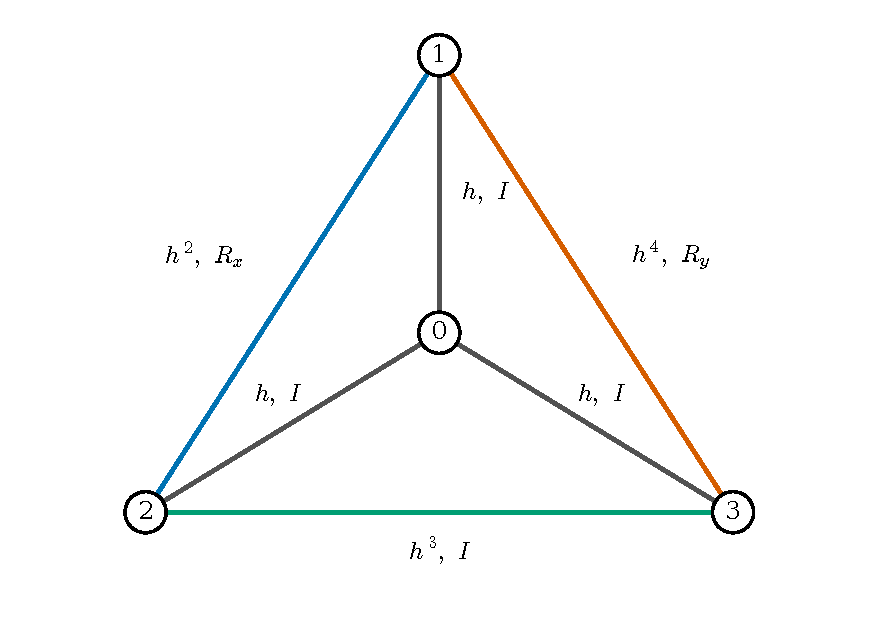
\includegraphics[width=.82\textwidth]{figures/output/three-scales.pdf}
 \caption{The actual attachment graph for the three-scale family.
 Each edge is labelled by its capacity weight and adjoint transport.
 The displayed transport on an edge $ij$, $i<j$, is from $j$ to $i$.
 The matrices $R_x,R_y$ are defined in \eqref{eq:rotations}.}
 \label{fig:three-scales}
\end{figure}

\begin{proposition}\label{prop:three-scales}
The twelve weak eigenvalues along this path satisfy
\begin{equation}\label{eq:three-scales}
 \begin{aligned}
 \lambda_0&\sim\tfrac12h^4,&
 \lambda_1,\lambda_2&\sim\tfrac12h^2,\\
 \lambda_3,\ldots,\lambda_8&\sim h,&
 \lambda_9,\lambda_{10},\lambda_{11}&\sim4h,
 \qquad \lambda_{12}\ge\gamma>0 .
 \end{aligned}
\end{equation}
Each member of a displayed group has the stated
asymptotic.
\end{proposition}
\begin{proof}
In three-by-three blocks the finite mass matrix is
$I_{12}$ and the energy matrix is
\begin{equation}\label{eq:three-scale-matrix}
 Q_h=\begin{pmatrix}
 3hI&-hI&-hI&-hI\\
 -hI&(h+h^2+h^4)I&-h^2R_x&-h^4R_y\\
 -hI&-h^2R_x^T&(h+h^2+h^3)I&-h^3I\\
 -hI&-h^4R_y^T&-h^3I&(h+h^3+h^4)I
 \end{pmatrix}.
\end{equation}
The order-$h$ star form has a three-dimensional kernel
$K=\{(x,x,x,x)\}$ and positive eigenvalues $1$ with
multiplicity six and $4$ with multiplicity three.
Thus nine eigenvalues have the asserted order-$h$
coefficients. The orthonormal embedding of $K$ is
$x\mapsto(x,x,x,x)/2$, and compression of the
order-$h^2$ coefficient is
\[
 \tfrac14(I-R_x)^T(I-R_x)
 =\operatorname{diag}(0,\tfrac12,\tfrac12).
\]
Trials in $K$ bound the remaining three eigenvalues
by $O(h^2)$. At such spectral parameters the
$K^\perp$ block is $hA+O(h^2)$ with $A>0$, and
its inverse is $O(h^{-1})$. The cross block is
$O(h^2)$, so its Schur contribution is $O(h^3)$.
Two eigenvalues are therefore asymptotic to $h^2/2$,
and one is $o(h^2)$.

The matrix is positive definite for $h>0$: zero
energy first forces a common vertex value, which
must be fixed by both $R_x$ and $R_y$; their fixed
axes meet only at zero. Direct expansion of the
printed matrix gives
\begin{equation}\label{eq:three-scale-det}
 \begin{split}
 \det Q_h=4h^{17}\big(&2+4h+14h^2+36h^3+55h^4+118h^5
                  +145h^6\\
                  &+194h^7+225h^8+178h^9+177h^{10}
                    +78h^{11}+54h^{12}\big).
 \end{split}
\end{equation}
The product of the nine fast eigenvalues is
asymptotic to $64h^9$, and that of the two middle
eigenvalues to $h^4/4$. Dividing the determinant by
these products gives $h^4/2$ for the remaining
eigenvalue. The relative comparison
\eqref{eq:relative-spectrum} transfers all these
coefficients to the actual operator.
\end{proof}

The accompanying exact calculation also verifies the
three rescaled characteristic-polynomial limits. For
$P(\lambda,h)=\det(\lambda I-Q_h)$ they are
\[
 \begin{aligned}
 h^{-12}P(hz,h)&\longrightarrow z^3(z-1)^6(z-4)^3,\\
 h^{-15}P(h^2z,h)&\longrightarrow-16z(2z-1)^2,\\
 h^{-17}P(h^4z,h)&\longrightarrow-8(2z-1).
 \end{aligned}
\]
These checks agree with the compression and determinant
argument above.

The inverse eigenvalue scales in
\eqref{eq:three-scales} are linearized relaxation
times. In particular, the weakest scale is not a
nonlinear tracking conclusion. In this example
$L_*=2\pi/h$ and $L_*\nu_0\sim\pi h^3\to0$,
so the all-time hypothesis in
Theorem~\ref{thm:all-time} below fails.

\section{The finite metric evolution}\label{sec:finite-flow}

Let $\cP_r$ be the positive Hermitian determinant-one
matrices, with metric
$g_P(V,W)=\tr(P^{-1}VP^{-1}W)$. Its distance and geodesic are
\begin{equation}\label{eq:matrix-geometry}
 \begin{split}
 d(P,Q)^2&=\tr\!\left(\log(P^{-1/2}QP^{-1/2})^2\right),\\
 \Geo(P,Q;\theta)&=P^{1/2}
 \exp\!\left(\theta\log(P^{-1/2}QP^{-1/2})\right)P^{1/2}.
 \end{split}
\end{equation}
This is a complete simply connected symmetric space of
nonpositive curvature; see \cite[Sections~2.3--2.6]{bhatia}.
Unitary congruences act isometrically and fix $I$.
On $\cP_r^4$ use the product metric with weights $A_i$.
With physical weights \eqref{eq:weights}, define
\begin{equation}\label{eq:finite-potential}
 \Phi_{\tau,U}(\mathbf H)
 =\frac12\sum_{e=ij}w_e
          d(H_i,U_{ij}H_jU_{ij}^*)^2.
\end{equation}

\begin{proposition}\label{prop:finite-flow}
The negative gradient flow of \eqref{eq:finite-potential} is
\begin{equation}\label{eq:finite-flow}
 H_i^{-1}\dot H_i=\frac1{A_i}\sum_{e=ij}w_e B_{ij},
 \qquad B_{ij}=\log(H_i^{-1}U_{ij}H_jU_{ij}^*).
\end{equation}
For initial tuples in a fixed bounded ball, it exists for all
physical times $s\ge0$ and remains in a compact matrix range
independent of $\tau,U$. Distances between two such solutions
with the same parameters are nonincreasing. On that range the
vector field and every fixed-order tuple derivative are
$O(L_*^{-1})$, uniformly in all length ratios and $U$.
\end{proposition}
\begin{proof}
The gradient of $\frac12d(P,Q)^2$ with respect to $P$
is $-\Log_PQ=-P\log(P^{-1}Q)$. Summing the incident
terms and dividing by $A_i$ gives \eqref{eq:finite-flow}.
Each $B_{ij}$ is $H_i$-self-adjoint and trace free,
so the velocity is tangent to $\cP_r$. The reverse
identity is $B_{ji}=-U_{ij}^*B_{ij}U_{ij}$; no
commutation of the endpoint metrics is used.

Squared distance is jointly geodesically convex on
this Hadamard manifold. Hence $\Phi$ is convex and
vanishes at $\mathbf I=(I,I,I,I)$. If $D_A$ is the
weighted product distance, gradient-flow convexity gives
\begin{equation}\label{eq:finite-confinement}
 \frac d{ds}\frac12D_A(\mathbf H,\mathbf I)^2
 \le-\Phi(\mathbf H).
\end{equation}
Closed bounded subsets are compact, so the smooth
vector field continues for all time. Applying the
same convexity inequality at the two endpoints of
the joining geodesic proves nonexpansion between
two solutions. Finally \eqref{eq:finite-flow} is a
finite sum of smooth matrix functions with coefficients
$w_e\le2\pi/L_*$. All tuple derivatives are bounded
on the confined range, uniformly in the compact
unitary parameter space. In particular
$|\dot B_{ij}|\le C/L_*$.
\end{proof}

The zero set of $\Phi$ consists of compatible metric
tuples. On irreducible unitary representations this set
is $\{\mathbf I\}$ by Schur's lemma and determinant
one. On reducible representations it is generally
positive-dimensional.

\begin{lemma}\label{lem:finite-coercivity}
Put $S_i=\log H_i$ and $R_f=\sum_iA_i\|S_i\|^2$.
Then
\[
 \Phi(\mathbf H)\ge\tfrac12Q_{\tau,U}(S)
 \ge\tfrac12\nu_0R_f,\qquad
 R_f(s)\le e^{-\nu_0s}R_f(0).
\]
\end{lemma}
\begin{proof}
The exponential map at $I$ expands distances in this
nonpositively curved symmetric space. Since unitary
congruence commutes with the exponential,
$d(H_i,UH_jU^*)\ge\|S_i-US_jU^*\|$.
This proves the energy inequalities. Moreover
$R_f=D_A(\mathbf H,\mathbf I)^2$, so
\eqref{eq:finite-confinement} gives
$R_f'\le-2\Phi\le-\nu_0R_f$.
\end{proof}

The finite equation has the same linearization
$\dot X=-B_{\tau,U}X$ as the effective spectral
operator. Its nonlinear variables need not commute.
For Example~\ref{ex:noncommuting}, no fixed simultaneous
diagonalization of the cycle transports reduces the
equation to independent scalar vertex equations.

\section{Reconstruction and the actual HYM flow}\label{sec:actual-flow}

The base and bundle parameters are fixed throughout
this section. All exact initial metrics are smooth,
have the parallel determinant, and obey fixed positive
bounds against $h_0$. In local unitary flat frames,
these conditions mean $\det H=1$ and $cI\le H\le CI$.
We use physical time $s$ and the normalization
\begin{equation}\label{eq:hym}
 H^{-1}\partial_sH=-2i\Lambda_{\omega_\tau}F_H.
\end{equation}
For $\omega_\tau=(i/2)a\,dz\wedge d\bar z$ this reads
\begin{equation}\label{eq:local-hym}
 \partial_sH=4a^{-1}
     (H_{z\bar z}-H_{\bar z}H^{-1}H_z).
\end{equation}
The scalar nonnegative Laplacian is
$\Delta_\tau=-4a^{-1}\partial_z\partial_{\bar z}$.
The real-coordinate expression is
\begin{equation}\label{eq:real-hym}
 \begin{split}
 a\partial_sH={}&H_{xx}+H_{yy}-H_xH^{-1}H_x-H_yH^{-1}H_y\\
 &+i(H_xH^{-1}H_y-H_yH^{-1}H_x).
 \end{split}
\end{equation}
The last term need not vanish. We retain it in every
curvature calculation.

For two metrics put
\[
 \sigma(H,K)=\tr(H^{-1}K+K^{-1}H)-2r.
\]
This is intrinsic under the bundle transition maps.
If $e^{b_j}$ are the eigenvalues of $H^{-1}K$, then
$d(H,K)^2=\sum_jb_j^2\le
\sum_j(e^{b_j}+e^{-b_j}-2)=\sigma(H,K)$.
For a smooth comparison metric define
\begin{equation}\label{eq:residual}
 \mathcal R(K)=K^{-1}\partial_sK+2i\Lambda F_K,
\end{equation}
measured in the operator norm induced by $K$.

\begin{lemma}\label{lem:trace-comparison}
The exact solution of \eqref{eq:hym} exists for all
$s\ge0$ and preserves its determinant and bounds
$ch_0\le H\le Ch_0$. For any smooth comparison
$K(s)$ with common positive bounds, one has
\begin{equation}\label{eq:trace-comparison}
 \int\sigma(H(s),K(s))
 \le\int\sigma(H(0),K(0))
       +C_0\int_0^s\!\int|\mathcal R(K(v))|_{\op}\,dA_\tau\,dv .
\end{equation}
Here and below unlabelled spatial integrals use $dA_\tau$.
The constant depends only on rank and the positive
bounds, not on a spectral gap or Sobolev constant.
\end{lemma}
\begin{proof}
Smooth all-time existence on a fixed compact base is
the classical metric heat-flow result
\cite{donaldson}; our normalization and order
preservation are also given in
\cite[Section~4.1 and Proposition~4.3]{hkkp}.
Apply order preservation to the stationary metrics
$ch_0,Ch_0$. The logarithm of the determinant satisfies
the scalar heat equation, so its constant initial
value is preserved.

For completeness the local Donaldson trace calculation
has the forced form, with $q=H^{-1}K$,
\[
 (\partial_s+\Delta_\tau)\sigma(H,K)
 \le\tr((q-q^{-1})\mathcal R(K)).
\]
For two exact velocities choose a holomorphic frame
normal for $H$ at the point. The curvature and
Laplacian terms in the forward trace cancel, leaving
$-4a^{-1}\tr(K_{\bar z}K^{-1}K_z)\le0$.
Interchange the metrics for the inverse trace.
The additional velocity $K\mathcal R(K)$ contributes
$\tr(q\mathcal R)$ and $-\tr(\mathcal Rq^{-1})$,
respectively. Both $q$ and $\mathcal R$ are
$K$-self-adjoint, and the common bounds control
$\tr q+\tr q^{-1}$. This proves the scalar inequality
with right-hand side at most $C_0|\mathcal R|_{\op}$.
Integration on the whole closed fibre removes the
Laplacian and gives \eqref{eq:trace-comparison}.
The calculation is unchanged by constant unitary
transition maps.
\end{proof}

Write $\varepsilon_e=L_e^{-1}$,
$\varepsilon_*=L_*^{-1}$, and
\begin{equation}\label{eq:error-scale}
 e_*=\frac{(1+\log L_*)^2}{L_*}.
\end{equation}
The initial tuples for \eqref{eq:finite-flow} lie in
a fixed bounded ball.

\begin{theorem}\label{thm:tracking}
For all sufficiently large $L_*$ there is a smooth
determinant-one comparison metric $\widehat K(s)$,
defined for all $s\ge0$ from the finite trajectory
\eqref{eq:finite-flow}, with uniform positive bounds
and
\begin{equation}\label{eq:residual-bound}
 \sup_{s\ge0}\int|\mathcal R(\widehat K(s))|_{\op}
 \le C L_*^{-2}(1+\log L_*)^2.
\end{equation}
On every fixed compact subset of component $i$,
$d(\widehat K(s),H_i(s))\le C_K/L_*$ uniformly in
$s$. If an exact flow has initial discrepancy
$\eta=\int\sigma(H^{\mathrm{in}},\widehat K(0))$,
then, for every $T\ge0$,
\begin{equation}\label{eq:tracking}
 \sup_{0\le s\le TL_*}\int
 d(H(s),\widehat K(s))^2\le\eta+CTe_*.
\end{equation}
The constants are independent of $T$, all positive
length ratios and all unitary parameters. Uniform
convergence over a class of initial metrics requires
uniform $\eta\to0$.
\end{theorem}

\subsection{Component potentials}
Let $g_{ie}$ be the mean-zero scalar Green function
on the fixed closed component $C_i$, normalized by
\[
 \Delta_i g_{ie}=-2\pi\delta_{p_{ie}}+\frac{2\pi}{A_i},
 \qquad g_{ie}=\log|u_e|+\gamma_{ie}(u_e)
\]
near the incidence. The regular part $\gamma_{ie}$
is smooth. Define
\begin{equation}\label{eq:component-correction}
 h_i=-\sum_{e=ij}\varepsilon_e B_{ij}g_{ie},
 \qquad K_i=H_i\exp(h_i).
\end{equation}
The logarithm $h_i$ is trace free and $H_i$-self-adjoint.
Away from the punctures,
\begin{equation}\label{eq:cancellation}
 \Delta_i h_i=-H_i^{-1}\dot H_i.
\end{equation}
Cut the components at radius $\rho=\varepsilon_*$.
Since $\max|\tau_e|=e^{-L_*}\ll\rho^2$, the two
branches of each node are disjoint there.
Fixed Green-function estimates and
Proposition~\ref{prop:finite-flow} give
\begin{equation}\label{eq:green-bounds}
 \begin{aligned}
 \|h_i\|_\infty&\le C\varepsilon_*(1+|\log\rho|),
 &\int|h_i|&\le C\varepsilon_*,
 &\int|h_i|^2&\le C\varepsilon_*^2,\\
 \int|\nabla h_i|^2&\le C\varepsilon_*^2(1+|\log\rho|),
 &\int|\dot h_i|&\le C\varepsilon_*^2,
 &\int|h_i||\Delta_i h_i|&\le C\varepsilon_*^2 .
 \end{aligned}
\end{equation}
In particular the integral bounds use integrability
of $\log|u|$ and its square, not their suprema on
the truncated domain. The time derivative estimate
uses $|\dot B_{ij}|\le C\varepsilon_*$ and
$\varepsilon_e\le\varepsilon_*$.

The exact exponential identity
\[
 e^{-h}\partial e^h
 =\int_0^1e^{-th}(\partial h)e^{th}\,dt
\]
and its time analogue show, after
\eqref{eq:cancellation}, that
\[
 |\mathcal R(K_i)|
 \le C\big(
 |\dot h_i|+\varepsilon_*|h_i|
 +|\nabla h_i|^2+|h_i||\Delta_i h_i|\big).
\]
Indeed the linear spatial term is $\Delta_i h_i$;
all terms produced by differentiating the conjugations
contain either two first derivatives or $h_i$ times
a second derivative. The time conjugation of
$H_i^{-1}\dot H_i$ contributes
$O(\varepsilon_*|h_i|)$. These identities include
the commutators in \eqref{eq:real-hym}. Integrating
\eqref{eq:green-bounds} bounds the residual by
$C\varepsilon_*^2(1+|\log\rho|)$ on the fixed
component. Transfer to the actual exterior costs
$Cb\rho^{-N}$, where $b=e^{-L_*}$, by
Lemma~\ref{lem:ambient}. A fixed $N$ suffices for
the finite derivative order involved.

\subsection{Node profiles and mixed weights}
Near an incidence write
\[
 h_i=-\varepsilon_eB_{ij}\log|u_e|+c_{ie}+q_{ie}(u_e),
 \qquad q_{ie}(0)=0.
\]
The regular terms include contributions from every
incident edge. Uniformly on the collar,
$|c_{ie}|\le C\varepsilon_*$ and
$|D^kq_{ie}|\le C\varepsilon_*\rho^{1-k}$
for $k\le2$. Their time derivatives gain
a factor $\varepsilon_*$.
Set $P_{ie}=H_i\exp(c_{ie})$. In the $i$ frame
the node metric is
\begin{equation}\label{eq:node-profile}
 N_e(s,u_e)=
 \Geo(P_{ie},U_{ij}P_{je}U_{ij}^*;
                  -\varepsilon_e\log|u_e|).
\end{equation}
The reverse branch has parameter
$1+\varepsilon_e\log|u_e|$, because $u_ev_e=\tau_e$.
Geodesic reversal and equivariance under unitary
congruence therefore give exactly the same metric
in the other frame. The individual $\varepsilon_e$
is essential for this compatibility.

At fixed time a geodesic in
\eqref{eq:node-profile} is $P\exp(\theta B)$
with a fixed matrix $B$ and harmonic scalar
$\theta$. Its Chern curvature is zero on the
annulus. Its time derivative is $O(\varepsilon_*)$
on the bounded endpoint range; the middle region
has area $O(\rho^2)$, so its integrated time
residual is $O(\varepsilon_*\rho^2)$.

On $\rho\le|u_e|\le2\rho$ use relative logarithms
$\ell_i(K)=\log(H_i^{-1}K)$.
For fixed endpoint metrics $H_i,H_j$, and
small self-adjoint endpoint logarithms $C_i,C_j$,
define the difference
\[
 \mathcal D(C_i,C_j;\theta)
 =\ell_i\!\left(\Geo(H_i e^{C_i},
              U_{ij}H_j e^{C_j}U_{ij}^*;\theta)\right)
                 -C_i-\theta B_{ij}.
\]
Self-adjointness here is with respect to
$H_i$ and $H_j$, respectively.
With no endpoint correction the node logarithm
is exactly $\theta B_{ij}$, so
$\mathcal D(0,0;\theta)=0$. At $\theta=0$
the geodesic equals $H_i e^{C_i}$, so
$\mathcal D(C_i,C_j;0)=0$.
The geodesic and logarithm are smooth on the
confined endpoint range. Integrating their
bounded mixed derivatives first along
$q(C_i,C_j)$, $0\le q\le1$, and then from
$0$ to $\theta$ gives
\[
 |\mathcal D(C_i,C_j;\theta)|
       \le C(|C_i|+|C_j|)|\theta|.
\]
Its first two $\theta$ derivatives are bounded
by $C(|C_i|+|C_j|)$, since they also vanish
when both corrections are zero.

Apply this with $C_i=c_{ie}$, $C_j=c_{je}$
and $\theta=-\varepsilon_e\log|u_e|$.
The endpoint corrections are $O(\varepsilon_*)$,
whereas the spatial derivatives of $\theta$
have size $O(\varepsilon_e\rho^{-k})$
for $k=1,2$. Thus the correction to the node
logarithm is bounded, through two spatial
derivatives, by
$C\varepsilon_*\varepsilon_e
(1+|\log\rho|)\rho^{-k}$.
The component logarithm differs from
$c_{ie}+\theta B_{ij}$ by the regular term
$q_{ie}$, whose corresponding bound is
$C\varepsilon_*\rho^{1-k}$.
Combining the two estimates gives
\begin{equation}\label{eq:mixed-collar}
 |D^k(\ell_i(K_i)-\ell_i(N_e))|
 \le C\left(
 \varepsilon_*\rho^{1-k}
 +\varepsilon_*\varepsilon_e(1+|\log\rho|)\rho^{-k}
 \right),\qquad k=0,1,2.
\end{equation}
The endpoint correction uses all incident weights,
whereas the node slope uses $\varepsilon_e$.
No inverse of $\varepsilon_e$ enters.

Join these logarithms with a fixed rescaled radial
cutoff and exponentiate relative to $H_i$. This
preserves positivity and determinant one. If $n$
is the node logarithm and $\delta$ is its cutoff
difference from the component logarithm, the full
curvature difference is bounded by
\[
 C\big(
 |D^2\delta|+|Dn||D\delta|
 +|\delta|(|D^2n|+|Dn|^2)+|D\delta|^2
 \big).
\]
Here $|Dn|\le C\varepsilon_e/\rho$ and
$|D^2n|\le C\varepsilon_e/\rho^2$.
Multiply by the collar area $O(\rho^2)$ and
substitute \eqref{eq:mixed-collar}. The integrated
curvature error is at most
\[
 C\big(\varepsilon_*\rho+
       \varepsilon_*\varepsilon_e(1+|\log\rho|)^2\big).
\]
Time terms contribute $O(\varepsilon_*\rho^2)$.
Terms of higher order are absorbed since
$\varepsilon_*|\log\rho|\to0$. The same geometric
transfer estimate contributes $Cb\rho^{-N}$.

\begin{proof}[Proof of Theorem~\ref{thm:tracking}]
Use \eqref{eq:component-correction},
\eqref{eq:node-profile} and the logarithmic cutoffs
to define one global $\widehat K(s)$ for the
entire finite trajectory. Their agreement under
the actual transition matrices proves that this
is a metric on $E_U$, not just a collection of
matrices. The confined endpoint range and the
small component logarithms give uniform positive
bounds. On each fixed component compact subset
$h_i=O(\varepsilon_*)$.

Sum the component, middle-node and collar estimates
with $\rho=\varepsilon_*$. The exponentially small
$e^{-L_*}L_*^N$ is absorbed by
$L_*^{-2}(1+\log L_*)^2$. All constants are
uniform for $s\ge0$, because the finite trajectory
stays in one compact range. This proves
\eqref{eq:residual-bound}.
Lemma~\ref{lem:trace-comparison} on the whole
closed fibre then gives \eqref{eq:tracking}
after integration to $TL_*$ and the inequality
$d^2\le\sigma$.
\end{proof}

\subsection{A uniform all-time conclusion}
\begin{theorem}\label{thm:all-time}
Under the hypotheses of Theorem~\ref{thm:tracking},
suppose in addition that
\begin{equation}\label{eq:rate-condition}
 L_*\nu_0\ge\kappa>0.
\end{equation}
Then, for sufficiently large $L_*$,
\[
 \sup_{s\ge0}\int d(H(s),\widehat K(s))^2
 \le C\eta+C_\kappa e_*(1+|\log e_*|).
\]
This is absolute tracking in the indicated norm.
\end{theorem}
\begin{proof}
For the exact solution set
$\mathcal F(H)=\int(\tr(h_0^{-1}H)-r)$.
Since $S=\log(h_0^{-1}H)$ is trace free and the
metrics have fixed positive bounds,
$\mathcal F$ is uniformly comparable to
$\int|S|^2=\int d(H,h_0)^2$. Taking the trace
of \eqref{eq:local-hym} and integrating gives
\[
 -\mathcal F'
 =4\int\tr(H_{\bar z}H^{-1}H_z)\,dx\,dy
 \ge c_1\int|D_UH|^2\,dA_\tau .
\]
Here $H_{\bar z}=H_z^*$. Replace $H^{-1}$ by
its uniform lower bound before using
$4\tr(H_z^*H_z)=\tr(H_x^2+H_y^2)$.
This does not discard a weighted commutator.
The derivative of the matrix logarithm is bounded
on the common matrix range, and hence
$|D_US|\le C|D_UH|$. Theorem~\ref{thm:spectrum}
and \eqref{eq:rate-condition} imply
$\lambda_0\ge\kappa/(2L_*)$ and therefore
\[
 -\mathcal F'\ge c_2\lambda_0\mathcal F,\qquad
 \int d(H(L_*\sigma),h_0)^2
       \le C e^{-c_3\kappa\sigma}.
\]

Lemma~\ref{lem:finite-coercivity} supplies the
corresponding exponential tail for the finite
trajectory. The reconstruction vanishes at
$\mathbf H=\mathbf I$ and is uniformly Lipschitz
from the confined tuple range to global $L^2$:
on components this follows from the Green
construction and on nodes from smoothness of
bounded geodesics. Its squared distance from
$h_0$ has the same type of exponential tail.
For $0\le s\le TL_*$ use \eqref{eq:tracking};
for $s\ge TL_*$ use the two tails and the
triangle inequality. Choosing
$T=C_\kappa(1+|\log e_*|)$ proves the estimate.
\end{proof}

The condition \eqref{eq:rate-condition} permits
some arbitrarily weak edges. In rank two keep
$01,02,03,12,13$ comparable to $w_*$, with the
two noncommuting transports of
Example~\ref{ex:noncommuting}, and let $23$
have any smaller positive weight. The first
five edges already have zero trace-free
kernel and a positive normalized gap; the
last nonnegative term cannot decrease it.
In contrast, Proposition~\ref{prop:three-scales}
does not satisfy \eqref{eq:rate-condition}.
On its weakest time $h^{-4}$ the accumulated
bound in \eqref{eq:tracking} is not small.
Uniform nonlinear tracking on that time
requires an additional argument.

\section{Spatial initial metrics and the initial layer}\label{sec:entry}

The initial-error hypothesis of Theorem~\ref{thm:tracking}
can be obtained from spatially varying metrics on the
normalization components. We first select the constant
metric determined by the actual flow on each fixed
component. We then construct an initial layer on the
smooth fibre whose duration is negligible compared
with $L_*$.

\subsection{Constant limits on a fixed component}
Let $Y$ be a fixed connected compact Riemann surface
of area $A$, with its trivial holomorphic rank-$r$
bundle and fixed flat frame. Write
$\langle f\rangle=A^{-1}\int_Y f\,dA$, entrywise
for a matrix. Let $\lambda_1>0$ be the first
positive scalar eigenvalue.
When a component flow converges to a constant
metric $P$, we call $P$ the asymptotic phase
of its initial metric.

\begin{theorem}\label{thm:component-phase}
For a smooth determinant-one initial metric with
$cI\le H^{\mathrm{in}}\le CI$, $0<c\le1\le C$,
the actual HYM flow converges to a unique constant
matrix $P=P(H^{\mathrm{in}})\in\cP_r$.
Set
\[
 M(s)=\langle H(s)\rangle,\quad J(s)=\log\det M(s),
 \quad V(s)=\langle\|H(s)-M(s)\|_{\HS}^2\rangle,
 \quad \gamma=2c^2C^{-2}\lambda_1 .
\]
Then $M$ decreases in Loewner order to $P$, and
\begin{equation}\label{eq:phase-entropy}
 \frac{V}{2C^2}\le J\le\frac{V}{2c^2},\quad
 J(s)\le J(0)e^{-\gamma s},\quad
 0\preceq M(s)-P,\quad \tr(M(s)-P)\le CJ(s).
\end{equation}
In particular
\begin{equation}\label{eq:phase-l2}
 \langle\|H(s)-P\|_{\HS}^2\rangle
 \le C^2(2J(0)+J(0)^2)e^{-\gamma s}.
\end{equation}
For $s\ge1$ the same exponential order bounds
$\sup_Y d(H(s),P)^2$, with a constant depending
only on $Y,c,C,r$. For two such initial metrics,
\begin{equation}\label{eq:phase-contraction}
 A\,\sigma(P(H^{\mathrm{in}}),P(K^{\mathrm{in}}))
 \le\int_Y\sigma(H^{\mathrm{in}},K^{\mathrm{in}})\,dA .
\end{equation}
\end{theorem}
\begin{proof}
Equation~\eqref{eq:local-hym} is
$H_s=-\Delta H-\mathcal A(H)$, with
$\mathcal A(H)=4a^{-1}H_z^*H^{-1}H_z\succeq0$.
Its spatial mean therefore satisfies
$M'=-\langle\mathcal A(H)\rangle\preceq0$.
Since $cI\le M\le CI$, it has a positive matrix
limit $P$. At this point its determinant has
not been prescribed.

For a Hermitian direction $Z$ and a matrix
$cI\le B\le CI$,
\[
 -D^2(\log\det)_B[Z,Z]
 =\tr(B^{-1}ZB^{-1}Z),\qquad
 C^{-2}\|Z\|^2\le\tr(B^{-1}ZB^{-1}Z)
                  \le c^{-2}\|Z\|^2.
\]
Diagonalizing $B$ proves the inequalities
entrywise. Apply Taylor's integral remainder
along the segment from $M$ to $H(x)$, then
average. The linear term vanishes and
$\log\det H(x)=0$, giving the two bounds
for $J$ in \eqref{eq:phase-entropy}.

Using positivity twice gives
\[
 -J'=\tr(M^{-1}\langle\mathcal A(H)\rangle)
 \ge C^{-1}\langle\tr\mathcal A(H)\rangle
 \ge C^{-2}\langle|dH|^2\rangle.
\]
In the last step one first bounds $H^{-1}$
below and then uses the unweighted identity
$4a^{-1}\tr(H_z^*H_z)=|dH|^2$. The scalar
Poincar\'e inequality in each matrix coordinate
gives $\langle|dH|^2\rangle\ge\lambda_1V$.
Thus $J'\le-\gamma J$. In particular
$J\to0$, so continuity of determinant gives
$\det P=1$.

The segment from $P$ to $M$ is bounded above
by $CI$. Since $M-P\succeq0$,
\[
 J=\int_0^1\tr\!\left[
 (P+t(M-P))^{-1}(M-P)\right]dt
 \ge C^{-1}\tr(M-P).
\]
The mean-zero cross term in the squared norm
vanishes, and therefore
\[
 \langle\|H-P\|^2\rangle
 =V+\|M-P\|^2\le2C^2J+C^2J^2.
\]
This proves \eqref{eq:phase-l2}.

The constant $P$ is itself an exact solution.
The scalar trace comparison shows that
$\sigma(H(s),P)$ is a nonnegative heat
subsolution. On the fixed component the
time-one heat kernel is bounded, whence
\[
 \sup_Y\sigma(H(s),P)
 \le C_Y\int_Y\sigma(H(s-1),P)\,dA
 \quad(s\ge1).
\]
On the fixed matrix range $\sigma$ is
comparable to squared matrix difference,
so \eqref{eq:phase-l2} proves uniform
convergence with the asserted rate.
Finally apply trace contraction to two
exact flows and pass to their uniform
constant limits. This gives
\eqref{eq:phase-contraction}.
\end{proof}

The phase depends on the entire spatial initial
metric. For diagonal initial data
$\operatorname{diag}(e^{f_1},\ldots,e^{f_r})$,
$\sum f_j=0$, it is
$\operatorname{diag}(e^{\langle f_1\rangle},
\ldots,e^{\langle f_r\rangle})$, by scalar
heat flow. No formula
$P=\exp\langle\log H^{\mathrm{in}}\rangle$
is asserted for general noncommuting data.
The contraction estimate makes the phase map
Lipschitz in $L^2$ on every fixed bounded
metric range.

\subsection{An open class on the smooth fibres}
Put $\rho=L_*^{-1}$ and let
$\Omega_i(2\rho)\subset C_i$ be the complement
of the incidence discs of radius $2\rho$.
Use the fixed exterior transfers and flat frames
of Section~\ref{sec:geometry}.
For a smooth trace-free $h_0$-Hermitian
endomorphism $S$ on $C_\tau$, fix $0<\beta<1$
and define
\begin{equation}\label{eq:extension-norm}
 \mathcal N_\tau(S)=\|S\|_{C^0(C_\tau)}
 +\inf_{\widetilde S_i|_{\Omega_i(2\rho)}=S_i}
             \sum_i\|\widetilde S_i\|_{C^{6,\beta}(C_i)} .
\end{equation}
The extensions are trace-free Hermitian matrices
in the component frames. Fix $R_0>0$ and take
$\mathcal N_\tau(S)<R_0$, with initial metric
$H^{\mathrm{in}}=h_0e^S$.
For each fixed smooth fibre this class is open
in the $C^{6,\beta}$ topology on smooth metrics:
fixed-domain extension operators bound
$\mathcal N_\tau(S_1-S_2)$ by a finite multiple
of the global $C^{6,\beta}$ norm.
Their operator norms need not be uniform as
$\rho\to0$. The radius in
\eqref{eq:extension-norm} is fixed independently
of the degeneration. Small fixed component
profiles joined smoothly on the nodes give
nonempty examples. Bounded smooth changes
inside the middle necks may have arbitrary
derivatives.

Choose extensions with total norm less than
$2R_0$. Apply Theorem~\ref{thm:component-phase}
to $e^{\widetilde S_i}$ and denote its flow by
$G_i(s,z)$ and selected phase by $P_i$.
All component flows have uniform positive
bounds and uniform exponential phase convergence.
Different admissible extensions agree outside
discs of area $O(\rho^2)$, so
\eqref{eq:phase-contraction} gives
$d(P_i,\widetilde P_i)=O(\rho)$.
Finite-flow nonexpansion preserves this
ambiguity at all later times.

\begin{theorem}\label{thm:entry}
For the class \eqref{eq:extension-norm} there
is a preparation time $s_*(\tau)\to\infty$,
uniform in all length ratios and unitary
parameters, such that $s_*/L_*\to0$.
Let $\widehat K_P(v)$ be the reconstruction
of Theorem~\ref{thm:tracking} for the finite
flow starting at the selected tuple $P$.
Then
\[
 \eta_*=\int\sigma(H(s_*),\widehat K_P(0))\to0
\]
uniformly over the stated initial class.
Consequently \eqref{eq:tracking} holds with
$H(s_*+v)$, $\widehat K_P(v)$ and initial
error $\eta_*$, for $0\le v\le TL_*$.
Under \eqref{eq:rate-condition} the all-time
estimate of Theorem~\ref{thm:all-time} holds
after the same preparation.
\end{theorem}
\begin{proof}
Fixed-base parabolic estimates for the component
flows with bounded $C^{6,\beta}$ initial profiles
give nondecreasing finite constants $C_n\ge1$
controlling the required space and time derivatives
on $0\le s\le n$. They depend on $R_0$ and the
fixed components, not on $\tau,U$.
Transfer $G_i(s,z)$ to the component exteriors.
On each node join its two point values
$G_i(s,p_{ie})$ and $U_{ij}G_j(s,p_{je})U_{ij}^*$
by the geodesic with parameter
$-\varepsilon_e\log|u_e|$. The node curvature
is zero, as in \eqref{eq:node-profile}.
On the $i$ collar use the spatially constant
reference $G_i(s,p_{ie})$ for both relative
logarithms. On $\rho\le|u_e|\le2\rho$, the difference
between the component and node logarithms, with
its first two derivatives, is at most
\[
 C_n(\rho+\varepsilon_e|\log\rho|)\rho^{-k},
 \qquad k=0,1,2 .
\]
The $O(\rho)$ term is the spatial variation
of $G_i$ from its nodal value, and the
other term is the small node parameter.
Use the same logarithmic cutoffs and
curvature-difference estimate as in
\eqref{eq:mixed-collar}. The integrated
collar residual is at most
$C_n(\rho+\varepsilon_*|\log\rho|)$.
The middle-node time residual is
$O(C_n\rho^2)$ and the geometric transfer
error is $O(C_nb\rho^{-N})$.
Thus the resulting global preparation
metric $K_{\mathrm{pre}}$ obeys
\[
 \sup_{0\le s\le n}\int|\mathcal R(K_{\mathrm{pre}})|
 \le C_n\delta_*,
 \qquad
 \delta_*=\frac{1+\log L_*}{L_*}+e^{-L_*}L_*^N\to0 .
\]
The initial metric and $K_{\mathrm{pre}}(0)$
agree outside regions of area $O(\rho^2)$
and have common positive bounds. By
\eqref{eq:trace-comparison} their integrated squared
distance, and their integrated trace
discrepancy, are bounded by
$C\rho^2+nC_n\delta_*$ up to time $n$.

For all sufficiently small parameters choose
\[
 s_*=\max\{n\in\mathbb N:nC_n\le\delta_*^{-1/2}\}.
\]
It tends to infinity because each $C_n$ is
finite, and it is finite because $C_n\ge1$.
Also $s_*\le\delta_*^{-1/2}$, which implies
$s_*/L_*\to0$. At that time the component
flows are exponentially close to $P_i$.
The reconstruction with initial tuple $P$
differs from the constant component metrics
by the Green corrections; their squared
integrals are $O(L_*^{-2})$. The remaining
node regions have area $O(\rho^2)$.
On the common matrix range, $\sigma$ is
comparable to squared distance and obeys
a triangle bound up to a fixed constant.
We obtain
\[
 \eta_*\le C_{R_0}\left(
 \sqrt{\delta_*}+e^{-\gamma_{R_0}(s_*-1)}
 +L_*^{-2}\right)\to0 .
\]
Restart Theorem~\ref{thm:tracking} at
$s_*$, and Theorem~\ref{thm:all-time} when
its additional rate hypothesis holds.
\end{proof}

For physical times after preparation one may align
the finite trajectory with time zero. Its speed
is $O(L_*^{-1})$, and the uniform $L^2$ Lipschitz
reconstruction gives, for $v\ge0$,
\[
 \int d(H(s_*+v),\widehat K_P(s_*+v))^2
 \le 2\int d(H(s_*+v),\widehat K_P(v))^2
       +C(s_*/L_*)^2 .
\]
Thus the time shift costs a fixed factor in the
preceding squared-error estimate and a vanishing
additional term. Uniform tracking does not
by itself assert convergence of a family of
selected phases. To pass to a fixed positive
rescaled-time limit, one must also assume
convergence of those phases and of the
normalized finite parameters.

\section{Component holonomy and neck degeneration}\label{sec:component-holonomy}

We next allow the component connections to vary.
The compact family in this section has one base
parameter and four necks of length $L+O(1)$.
The bundle parameters are independent of $L$.
The conclusions therefore concern arbitrary
component-to-neck scale ratios; they do not
combine varying component holonomy with the
six independent node parameters of
Section~\ref{sec:geometry}.

\subsection{A compact family and its flat bundles}
Let $E$ be the projective elliptic curve
$y^2=(x-1)(x-2)(x-3)$, with origin $o$ at infinity.
The sections $s_0=x$ and $s_1=1$ of
$\mathcal O_E(2o)$ have disjoint zero divisors
$p+q$ and $2o$. In $E\times\PP^1\times\Delta$ set
\begin{equation}\label{eq:elliptic-family}
 \cC=\{s_0uv+t s_1(u^2+v^2)=0\},
 \qquad \pi:\cC\longrightarrow\Delta .
\end{equation}
Give $E$ a fixed flat Kähler metric and $\PP^1$
a fixed smooth Kähler metric. Restrict their
product, with a positive disc term, to $\cC$.

\begin{proposition}\label{prop:elliptic-family}
After shrinking $\Delta$, \eqref{eq:elliptic-family}
is a proper projective semistable family with
smooth total surface and connected genus-three
smooth fibres. Its central components are two
copies $E_+,E_-$ of $E$ and two rational curves
$R_p,R_q$, with dual graph $K_{2,2}$.

Fix trace-free Hermitian matrices $T_i$ and
nonzero real harmonic one-forms $\omega_i$ on
$E_i$, for $i=+,-$. The component connections
\[
 D_i=d-i\alpha_iT_i\omega_i,\qquad \alpha_i\in\RR,
\]
the trivial connections on $R_p,R_q$, and arbitrary
node identifications $U_{ij}\in\SU(r)$ define
flat determinant-one bundles on a neighborhood
of the whole central fibre. For every fixed
$\alpha$ they are holomorphic bundles over the
restricted family, with parallel metric $h_0$.
Dependence on $\alpha$ is smooth and real.
\end{proposition}
\begin{proof}
At a node the equation is $xw+t(1+w^2)=0$.
Its derivative in $t$ is nonzero there.
Elsewhere on the central fibre a spatial
derivative is nonzero, including above $o$:
divide by $s_0$ and use that $s_1/s_0$ has a
double zero. Compactness gives a smooth total
surface after restriction. The projection is
proper and projective. Its fibres are effective
Cartier divisors, and the local map to the disc
is flat. The holomorphic Morse normal form
gives $ab=t$ at each node.

For $t\ne0$, projection to $E$ has degree two.
The discriminant in the affine chart is
$x^2-4t^2$, with four distinct simple zeros
for small $t$. At $o$ the equation
$w+t(s_1/s_0)(1+w^2)=0$ and its reciprocal
chart give two unramified points.
Thus $C_t$ is smooth. A disconnected
double cover would be unramified, so it is
connected. Riemann--Hurwitz gives genus three.

Use disjoint node bidiscs and component
exteriors as in Proposition~\ref{prop:bundle}.
Trivialize each exterior smoothly over the
disc, with the lifts agreeing with the branch
coordinate on its collars. Pull back
$\omega_i$ from the fixed punctured component.
It is closed and has zero puncture periods.
On an incidence collar write $\omega_i=dF_{ie}$,
with the central primitive normalized to
vanish at the node. The frame change
$G_{ie}=\exp(i\alpha_iT_iF_{ie})$ gives a
parallel unitary frame. Give each node bidisc
the trivial flat bundle and identify these
parallel frames by the prescribed constant
unitary maps. Only incidence overlaps occur;
there are no triple overlaps.

These are flat isomorphisms, so the connections
glue to a unitary flat connection with parallel
determinant. Its $(0,1)$ part is integrable.
The exterior smooth frames need not be
holomorphic; the local parallel frames are.
Properness permits a smaller disc on which
this neighborhood contains every whole fibre.
This proves the claimed total-family construction.
\end{proof}

Let $A_i$ be the four limiting areas and put
$\kappa_i=\int_{E_i}|\omega_i|^2$.
The elliptic limiting metrics are flat, so
$|\omega_i|^2=\kappa_i/A_i$ is constant.
All necks have leading capacity $2\pi/L$, where
$L=\log(1/|t|)$.

The distinction between node identifications
and based holonomy matters here.
Killing the annular core loops gives a
surjection
\[
 \pi_1(C_t)\longrightarrow
 \pi_1(E_+)*\pi_1(E_-)*\mathbb Z .
\]
Fix paths $c_{ie}$ from component basepoints
to the nodes and put
\[
 \mathcal U_{ie}=\exp\left(i\alpha_iT_i
                       \int_{c_{ie}}\omega_i\right),
 \qquad K_{ij}=\mathcal U_{ie}^{-1}U_{ij}\mathcal U_{je}.
\]
On rational components $\mathcal U_{ie}=I$.
Spanning-tree products of the $K_{ij}$ identify
the component basepoint fibres, and their cycle
product represents the chosen based graph loop.
A bare product of the $U_{ij}$ need not do so.
Changing paths changes the presentation of
the same local system.

For all sufficiently small $\alpha_i$, the
parallel trace-free Hermitian endomorphisms
are exactly the tuples satisfying
\begin{equation}\label{eq:coupled-kernel}
 X_i=\Ad(U_{ij})X_j,\qquad
 \alpha_i[T_i,X_i]=0\quad(i=+,-).
\end{equation}
Indeed, choose a nonzero period of $\omega_i$.
For small nonzero $\alpha_i$, exponentiation
does not identify distinct eigenvalues of
$T_i$ at this period. Its holonomy commutant
is therefore the commutant of $T_i$.
Such an endomorphism is constant in the
harmonic component gauge and unchanged by
each $G_{ie}$; node compatibility is precisely
\eqref{eq:coupled-kernel}. At $\alpha_i=0$
the component condition is vacuous.
The unitary correspondence \cite{narasimhan-seshadri} gives
polystability, and stability exactly when this
trace-free commutant is zero.

For example, take $r=2$, $T_+=\sigma_z$,
$\alpha_-=0$, and a harmonic form on $E_+$
with periods $(1,0)$. Set the tree maps to
$I$ and the remaining node map to
$W=(I+i\sigma_x)/\sqrt2$.
Tree compatibility makes all $X_i=X$.
When $\alpha_+\ne0$ is small the component
condition gives $X=c\sigma_z$, and
$W\sigma_zW^*=\sigma_y$ forces $c=0$.
The bundle is stable. At $\alpha_+=0$ the
representation is generated by $W$ and is
reducible. This is actual stable-to-polystable
variation, independent of $t$. It does not
produce an unstable locus or a topologically
nontrivial smooth $\SU(r)$ bundle on a curve.

\subsection{The coupled relative spectrum}
On $\cV=\bigoplus_{i=1}^4\Herm_0(r)$ define
\begin{equation}\label{eq:coupled-form}
 \begin{split}
 g_\alpha(X)&=\sum_{i=+,-}\alpha_i^2\kappa_i
                                  \|[T_i,X_i]\|_{\HS}^2,\\
 q_U(X)&=\sum_{e=ij}\|X_i-\Ad(U_{ij})X_j\|_{\HS}^2,\\
 Q_{t,\alpha,U}(X)&=g_\alpha(X)+\frac{2\pi}{L}q_U(X),
 \qquad M(X)=\sum_i A_i\tr(X_i^2).
 \end{split}
\end{equation}
Write $\alpha_*=\max_i|\alpha_i|$,
$m=4(r^2-1)$, and let $\nu_0,\ldots,\nu_{m-1}$
be the generalized eigenvalues of $(Q,M)$,
including zeros.

\begin{theorem}\label{thm:coupled-spectrum}
Let $\lambda_k$ be the eigenvalues of $D^*D$
on the real trace-free Hermitian endomorphisms
of the bundle in Proposition~\ref{prop:elliptic-family}.
As $(|t|,\alpha_*)\to(0,0)$,
\[
 (1-\epsilon)\nu_k\le\lambda_k\le(1+\epsilon)\nu_k
 \quad(0\le k<m),\qquad \epsilon\longrightarrow0,
\]
uniformly in all $U$. There is a uniform
complementary gap $\lambda_m\ge\gamma>0$
in a sufficiently small product neighborhood.
The exact kernel is \eqref{eq:coupled-kernel}.
No restriction is imposed on $\alpha_i^2L$
or on the distance to a reducible representation.
\end{theorem}
\begin{proof}
We give the component and matching estimates
that replace those of Section~\ref{sec:spectrum}.
On a closed elliptic component a constant
matrix has energy
$\alpha_i^2\kappa_i\|[T_i,X_i]\|^2$.
In flat coordinates the constant subspace is
invariant under $D_i^*D_i$. After diagonalizing
$T_i$, entry $ab$ on a dual-lattice Fourier
mode $k$ has eigenvalue
$|2\pi k-\alpha_i(\lambda_a(T_i)-\lambda_b(T_i))
\omega_i|^2$. The nonzero Fourier modes have
a uniform gap for small $\alpha_i$.

Fix a small radius $a>0$. A local primitive
$F$ satisfies $F(0)=0$, $|F|\le Ca$ and
$|dF|\le C$. On $a<|z|<2a$ join $X_i$ to
the parallel section $\Ad(e^{i\alpha_iT_iF})X_i$
with a radial cutoff. Since
\[
 \|\Ad(e^{i\alpha_iT_iF})X_i-X_i\|
 \le|\alpha_iF|\,\|[T_i,X_i]\|,
\]
this modification changes the component
energy by at most $Ca^2\alpha_i^2
\|[T_i,X_i]\|^2$. In the flat node frames
interpolate affinely in log radius over
$\ell_a=L+2\log a$.
For the resulting trial section $JX$,
\[
 \begin{split}
 E(JX)&\le(1+Ca^2+o_a(t))g_\alpha(X)
                         +\frac{2\pi}{\ell_a}q_U(X),\\
 |\|JX\|^2-M(X)|&\le(Ca^2+o_a(t))M(X).
 \end{split}
\]
Metric transfer errors are multiplicative
because the pulled-back connection is fixed.
These bounds give the relative upper
estimate and $\lambda_{m-1}\le
C(\alpha_*^2+L^{-1})$.

For the lower estimate, let $\Omega_a$ be a
punctured elliptic component and let $\omega_a$
be the absolute harmonic representative of
the class of $\omega|_{\Omega_a}$.
Thus $\omega_a$ is closed, coclosed, has zero
normal component, and
$\omega=\omega_a+df_a$. Write
$\kappa_a=\|\omega_a\|^2$. Then
$\kappa_a\to\kappa$ as $a\to0$.
Indeed $\omega$ is a competitor, so
$\kappa_a\le\kappa$. A bounded-energy weak
limit retains its periods and is harmonic
away from the punctures. An isolated
singularity of an $L^2$ harmonic one-form
on a surface is removable: even a simple
pole in its holomorphic Laurent expansion
has infinite $L^2$ norm. The limit is
therefore $\omega$, and lower
semicontinuity proves the assertion.

Gauge by $e^{i\alpha T f_a}$. For an entry
with eigenvalue difference $\delta$ of $T$,
the connection becomes $d-i\beta\omega_a$,
where $\beta=\alpha\delta$.
Write $v=z+w$, with $\int_{\Omega_a}w=0$.
The absolute boundary condition gives
$\langle dw,\omega_a z\rangle=0$.
For small $|\beta|$, Poincaré implies
$\|w\|\le C_a\|(d-i\beta\omega_a)w\|$.
The remaining cross term is bounded by
$C_a\beta^2|z|\|w\|$. Completing the square
therefore gives
\[
 \begin{split}
 \|(d-i\beta\omega_a)v\|^2
 &\ge\tfrac12\|(d-i\beta\omega_a)w\|^2
                +(\beta^2\kappa_a-C_a\beta^4)|z|^2,\\
 \|w\|_{H^1}^2+\beta^2|z|^2
 &\le C_a\|(d-i\beta\omega_a)v\|^2 .
 \end{split}
\]
These inequalities remain valid at $\beta=0$.
Summing entries defines component means $X_i$
and gives, with multiplicative $1+o_a(t)$
changes on the nearby fibre,
\[
 \begin{split}
 E_i&\ge(1-C_a\alpha_*^2)
                  \alpha_i^2\kappa_{i,a}\|[T_i,X_i]\|^2,\\
 \|w_i\|_{H^1}^2+\alpha_i^2\|[T_i,X_i]\|^2
 &\le C_a E_i.
 \end{split}
\]
On rational components take the ordinary mean.

The mean gauge and the parallel node frame
differ by $e^{i\alpha_iT_i(f_{i,a}-F_{ie})}$.
On a fixed collar its action on $X_i$ differs
from $X_i$ by at most
$C_a|\alpha_i|\|[T_i,X_i]\|$.
The trace bound on $w_i$ thus gives
$|c_{ie}-X_i|\le C_a E_i^{1/2}$ for the
parallel-frame boundary averages.
In particular there is no additive error
$O(\alpha_i)\|X_i\|$.
Separate the disjoint component and neck
energies as $E_{\mathrm c}$ and $E_{\mathrm n}$.
Angular averaging on the annuli yields
\[
 q_U(X)^{1/2}
 \le\sqrt{\ell_a/(2\pi)}\,E_{\mathrm n}^{1/2}
                                +C_aE_{\mathrm c}^{1/2}.
 \]
After multiplication by $\sqrt{2\pi/L}$ and
Young's inequality, this gives
\[
 \frac{2\pi}{L}q_U(X)
 \le(1+O_a(L^{-1/2}))E_{\mathrm n}
                              +O_a(L^{-1/2})E_{\mathrm c}.
\]
Combining it with the component estimate,
without counting either energy twice, gives
\begin{equation}\label{eq:coupled-lower}
 Q(X(s))\le
 \bigl(1+\theta(a)+C_a\alpha_*^2
              +O_a(L^{-1/2})+o_a(t)\bigr)E(s),
 \qquad \theta(a)\to0 .
\end{equation}

We also need the mass comparison. For a
normalized eigensection of eigenvalue
$\lambda\le1$, the preceding bounds give
$\|w_i\|_{H^1}\le C_a\sqrt\lambda$ and bounded
means. In the mean gauge the central operator
applied to $X_i$ is
$\alpha_i^2|\omega_{i,a}|^2\operatorname{ad}(T_i)^2X_i$,
bounded by $C_a|\alpha_i|\sqrt{E_i}$.
The metric perturbation adds at most
$o_a(t)|\alpha_i|\|[T_i,X_i]\|$.
Interior $W^{2,2}$ estimates on fixed enlarged
collars therefore control the boundary
values in $C^0$. The enlargement passes
slightly into the flat node chart and
introduces no shrinking-domain estimate.
Harmonic extension in that chart, followed
by Lemma~\ref{lem:zero-boundary} for its
zero-boundary remainder, rules out annular
mass loss. For a combination of at most
$m+1$ eigenvectors of eigenvalues at most
$\Lambda\le1$, the result is
\[
 |M(X(s))-\|s\|^2|
 \le(Ca^2+C_a\sqrt\Lambda+o_a(t))\|s\|^2 .
\]
This is the mass argument of
Lemma~\ref{lem:low-mass} with the
energy-controlled component gauges above.

If $\lambda_m$ tended to zero, these means
would inject an $(m+1)$-dimensional space
into $\cV$, a contradiction. The same mass
estimate and \eqref{eq:coupled-lower},
applied to the first $k+1$ eigensections,
give the relative lower estimate by min--max.
Choose $a$ first and then choose $|t|$ and
$\alpha_*$ independently small. This proves
uniformity for every ratio $\alpha_i^2L$.
Finally $Q=0$ is exactly
\eqref{eq:coupled-kernel}, already identified
with the actual parallel sections.
\end{proof}

\subsection{The exact component field}
For $H\in\cP_r$ set
$f_T(H)=\tr(TH^{-1}TH)-\tr(T^2)$.
In the smooth harmonic component frame a
spatially constant metric has
\[
 H^{-1}\partial_{D_i}H
 =-i\alpha_i(H^{-1}T_iH-T_i)\omega_i^{1,0},
 \qquad
 F_H=\alpha_i^2[T_i,H^{-1}T_iH]\,
                   \omega_i^{1,0}\wedge\omega_i^{0,1}.
\]
Since $2i\Lambda(\omega_i^{1,0}\wedge
\omega_i^{0,1})=|\omega_i|^2$, its exact
component HYM equation is
\[
 H^{-1}\dot H=-\alpha_i^2|\omega_i|^2[T_i,H^{-1}T_iH].
\]

Differentiation gives
$df_T(HS)=\tr([T,H^{-1}TH]S)$.
The gradient is $H$-self-adjoint and trace
free. It is geodesically convex: along
$H(u)=H_0^{1/2}e^{uK}H_0^{1/2}$, put
$B=H_0^{-1/2}TH_0^{1/2}$ and diagonalize
$K$ with eigenvalues $k_a$. Then
\[
 \tr(TH(u)^{-1}TH(u))
       =\sum_{a,b}|B_{ba}|^2e^{u(k_a-k_b)}.
\]
For $H=e^S$, the Hermitian symmetry of $T$
also gives
\[
 f_T(e^S)=2\sum_{a<b}|T_{ab}|^2
                      (\cosh(s_a-s_b)-1)
 \ge\tfrac12\|[T,S]\|^2,\qquad
 f_T(e^{uS})\le u^2f_T(e^S)\quad(0\le u\le1).
\]

Equip $\cP_r^4$ with the masses $A_i$ and
define
\[
 \Phi_{t,\alpha,U}(H)=\sum_{i=+,-}\alpha_i^2\kappa_i f_{T_i}(H_i)
        +\frac{\pi}{L}\sum_{e=ij}d(H_i,U_{ij}H_jU_{ij}^*)^2.
\]
Its negative gradient is
\begin{equation}\label{eq:coupled-flow}
 A_iH_i^{-1}\dot H_i
 =-\alpha_i^2\kappa_i[T_i,H_i^{-1}T_iH_i]
          +\frac{2\pi}{L}\sum_{j:ij}B_{ij},
 \qquad B_{ij}=\log(H_i^{-1}U_{ij}H_jU_{ij}^*),
\end{equation}
with the component term omitted on rational
vertices. All derivatives use physical time.

Convexity gives nonexpansion of this flow.
Radial contraction towards the identity
gives $\Phi_{t,\alpha,U}(e^{uS})\le u^2\Phi_{t,\alpha,U}(e^S)$,
and the distance-decreasing logarithm gives
$\Phi_{t,\alpha,U}(e^S)\ge Q(S)/2$.
Consequently
\begin{equation}\label{eq:coupled-decay}
 R(s):=\tfrac12 M(\log H(s))
 \le R(0)e^{-2\nu_0s}.
\end{equation}
Indeed $R'\le-2\Phi_{t,\alpha,U}\le-2\nu_0R$.
This also confines every trajectory to its
initial product ball and proves all-time
existence, including $\nu_0=0$.
On that ball its speed, and the physical
time derivative of any fixed smooth tuple
function, are bounded by $C\zeta$, where
$\zeta=\alpha_*^2+L^{-1}$.
The speed in neck time need not be bounded.

\subsection{Actual coupled tracking}
Put
\[
 e(t,\alpha)=\alpha_*+\frac{(1+\log L)^2}{L}.
\]
The base, component and gluing parameters
remain fixed during each trajectory.

\begin{theorem}\label{thm:coupled-tracking}
For $|t|$ and $\alpha_*$ independently
sufficiently small, and initial tuples in a fixed bounded ball,
the finite flow \eqref{eq:coupled-flow}
defines a smooth determinant-one comparison
metric $\widehat K(s)$ on $C_t$, for all
$s\ge0$, with uniform positive bounds and
\begin{equation}\label{eq:coupled-residual}
 \sup_{s\ge0}\int_{C_t}|\mathcal R(\widehat K(s))|_{\op}
 \le C\left(\frac{\alpha_*}{L}
                       +\frac{(1+\log L)^2}{L^2}\right).
\end{equation}
On each fixed compact component region,
in the harmonic gauge,
$d(\widehat K(s),H_i(s))\le C_K/L$.
For an actual HYM flow with fixed positive
initial bounds, let
$\eta=\int_{C_t}\sigma(H(0),\widehat K(0))$.
Then for every $T\ge0$,
\begin{equation}\label{eq:coupled-tracking}
 \sup_{0\le s\le TL}\int_{C_t}d(H(s),\widehat K(s))^2
                       \le\eta+CTe(t,\alpha).
\end{equation}
All constants are independent of $T$, $U$
and the ratios $\alpha_i^2L$.
If in addition $L\nu_0\ge\nu_*>0$, then
\begin{equation}\label{eq:coupled-alltime}
 \sup_{s\ge0}\int_{C_t}d(H(s),\widehat K(s))^2
 \le\eta+C_{\nu_*}e(t,\alpha)(1+|\log e(t,\alpha)|)
\end{equation}
for small $e(t,\alpha)$.
\end{theorem}
\begin{proof}
Use the component Green functions of
Section~\ref{sec:actual-flow} and set
\[
 \xi_i=-\sum_{e=ij}B_{ij}g_{ie},\qquad
 V_i=\frac{2\pi}{A_i}\sum_{j:ij}B_{ij},
 \qquad K_i=H_i e^{\varepsilon\xi_i},
 \quad \varepsilon=L^{-1}.
\]
Off the punctures $\Delta_i\xi_i=-V_i$.
On a component cut at radius $\rho/2$,
the fixed Green estimates give
\[
 \begin{gathered}
 \|\xi_i\|_\infty\le C(1+|\log\rho|),\qquad
 |\nabla^k\xi_i|\le C(1+|u|^{-k})\quad(k=1,2),\\
 \int(|\xi_i|+|\xi_i|^2+|\nabla\xi_i|)\le C,\qquad
 \int|\nabla\xi_i|^2\le C(1+|\log\rho|),\\
 \int|\xi_i|\,|\Delta_i\xi_i|\le C,\qquad
 \int|\dot\xi_i|\le C\zeta .
 \end{gathered}
\]
The derivative bound is written near each
node in its coordinate $u$; away from the
nodes it is uniform. The last estimate uses the physical speed
bound; no bound on $L\dot H_i$ is used.

In the harmonic gauge write $h=\varepsilon\xi_i$
and $C_H=H^{-1}\partial_{D_i}H$.
The exact identity
\[
 K^{-1}\partial_{D_i}K
       =e^{-h}C_He^h+e^{-h}\partial_{D_i}e^h
\]
and the integral formula for the derivative
of the exponential imply, when $|h|\le1$,
\[
 |2i\Lambda F_K-2i\Lambda F_H-\Delta_i h|
 \le C\bigl(
 |\alpha_i||\nabla h|+\alpha_i^2|h|
                +|\nabla h|^2+|h||\Delta_i h|\bigr).
\]
Here $|C_H|=O(|\alpha_i|)$ and its covariant
derivative is $O(\alpha_i^2)$.
The terms linear in $h$ contain either a
connection coefficient and a derivative of
$h$, or two connection coefficients and
$h$. Differentiating the exponential produces
the two quadratic terms. The time identity
$K^{-1}\dot K=e^{-h}(H^{-1}\dot H)e^h+
e^{-h}\partial_s e^h$ has error
$C(|\dot h|+\zeta|h|)$.
Since $|\omega_i|^2=\kappa_i/A_i$,
\eqref{eq:coupled-flow} cancels the leading
terms exactly:
\[
 H_i^{-1}\dot H_i+2i\Lambda_i F_{H_i}
                                +\varepsilon\Delta_i\xi_i=0.
\]
Thus the integrated component residual is
at most
\[
 C\{\varepsilon(\zeta+\alpha_*+\alpha_*^2)
                       +\varepsilon^2(1+|\log\rho|)\}.
\]
There is no uncancelled pure component
error of order $\alpha_*^4$.
Transfer to the smoothing adds
$C|t|\rho^{-N}$ for a fixed $N$.

At incidence $ie$ write
$\xi_i=-B_{ij}\log|u|+c_{ie}+q_{ie}(u)$,
where $q_{ie}(0)=0$, and put
$P_{ie}=H_i e^{\varepsilon c_{ie}}$.
In the node parallel frame use
\[
 N_e=\Geo(P_{ie},U_{ij}P_{je}U_{ij}^*;
                                          -\varepsilon\log|u|).
\]
Geodesic reversal and $uv=t$ give exact
compatibility from both ends.
This node metric has zero spatial Chern
curvature and physical time velocity
$O(\zeta)$, so its middle-node residual
has integral $O(\zeta\rho^2)$.

The component metric in this parallel
frame is $K_i^{\mathrm{par}}=G_{ie}^*K_iG_{ie}$,
where $G_{ie}=e^{i\alpha_iT_iF_{ie}}$ and
$F_{ie}(0)=0$. On the incidence annulus,
in the logarithm $\ell_i(K)=\log(H_i^{-1}K)$,
the endpoint expansion used in
\eqref{eq:mixed-collar} gives
\[
 |D^k(\ell_i(K_i^{\mathrm{par}})-\ell_i(N_e))|
 \le C\{\alpha_*\rho^{1-k}
       +\varepsilon\rho^{1-k}
       +\varepsilon^2(1+|\log\rho|)\rho^{-k}\},
 \quad k=0,1,2.
\]
The new first term comes from $G_{ie}-I$.
Each estimate differentiated in physical
time gains a factor $C\zeta$.
Interpolate the two $H_i$-self-adjoint,
trace-free logarithms and exponentiate.
The curvature-difference estimate of
Section~\ref{sec:actual-flow}, with
$|Dn|\le C\varepsilon/\rho$ and
$|D^2n|\le C\varepsilon/\rho^2$ for
$n=\ell_i(N_e)$, gives the integrated
collar bound
\[
 C\{\alpha_*\rho+\varepsilon\rho
       +\varepsilon^2(1+|\log\rho|)^2
       +\alpha_*^2\rho^2+\zeta\rho^2\}.
\]
Choose $\rho=L^{-1}$.
Then $\varepsilon|\log\rho|\to0$,
the exponentially small transfer error
is absorbed, and all pieces give
\eqref{eq:coupled-residual}.
They remain in a common positive matrix
range for all physical time.
On fixed component regions the Green
correction is $O(L^{-1})$.

Lemma~\ref{lem:trace-comparison} is local
in parallel holomorphic frames and
applies to this flat bundle. Integrating
\eqref{eq:coupled-residual} proves
\eqref{eq:coupled-tracking}, without a
factor exponential in $\alpha_*^2s$.

For the all-time statement,
Theorem~\ref{thm:coupled-spectrum} gives
$\lambda_0\ge\nu_*/(2L)$.
The actual trace coercivity used in
Theorem~\ref{thm:all-time} remains valid
in the local parallel frames:
for $H=e^S$ and $cI\le H\le CI$,
\[
 \frac c2\|S\|_{L^2}^2
 \le F:=\int\tr(H-I)\le\frac C2\|S\|_{L^2}^2,
 \qquad -F'\ge\frac{c^2}{C}\int|DS|^2 .
\]
It implies exponential decay in $s/L$
with rate bounded below by a multiple
of $\nu_*$. Equation~\eqref{eq:coupled-decay}
gives the same type of bound for the
finite flow. All correction coefficients
vanish at the identity tuple, which is
fixed by the component gauge changes.
The reconstructed metric consequently
has an exponential tail as well.
Combine these tails beyond time $TL$
with \eqref{eq:coupled-tracking} before
that time and take $T$ proportional to
$|\log e(t,\alpha)|$. This proves
\eqref{eq:coupled-alltime}.
\end{proof}

The additional rate condition is nonempty
even when $\alpha_*^2L\to\infty$.
For the rank-two example above write
$Q=hq+aP$, where $h=2\pi/L$,
$a=\alpha_+^2\kappa_+$ and
$P(X)=\|[\sigma_z,X_+]\|^2$.
The kernel computation gives
$\ker q\cap\ker P=0$.
If $a/h\ge\eta_0>0$, then
$Q\ge h(q+\eta_0P)$ and $L\nu_0$
has a positive lower bound.
As $a/h\to0$ that bound fails; the
bounded-neck-time theorem still applies.

\subsection{The initial layer with varying component holonomy}
Use the norm \eqref{eq:extension-norm} with
$\rho=L^{-1}$, the four components of
\eqref{eq:elliptic-family}, and the harmonic
component frames. Denote it by
$\mathcal N_{t,\alpha,U}$.
It again defines a fixed-radius nonempty
open class $\mathcal N_{t,\alpha,U}(S)<R_0$
on each smooth fibre, with only a $C^0$
bound imposed in the middle necks.
For admissible component extensions take
the phases $P_i$ of their \emph{trivial}
component flows from
Theorem~\ref{thm:component-phase}.

\begin{theorem}\label{thm:coupled-entry}
In the joint limit $(|t|,\alpha_*)\to(0,0)$,
there is a preparation time
$s_*(t,\alpha;R_0)\to\infty$ such that
$(\alpha_*^2+L^{-1})s_*\to0$ and
\[
 \eta_*=\int_{C_t}\sigma(H(s_*),\widehat K_P(0))
 \longrightarrow0
\]
uniformly over this initial class and
all unitary parameters.
The estimates of
Theorem~\ref{thm:coupled-tracking} apply
after $s_*$ with initial error $\eta_*$.
The finite flow may instead be aligned
with physical time zero at the cost of
a fixed factor in the squared error and
an additional $O((\zeta s_*)^2)$.
\end{theorem}
\begin{proof}
The preparation construction in
Theorem~\ref{thm:entry} uses trivial
component solutions $G_i(s,z)$ with
uniform derivative bounds $C_n$ on
$0\le s\le n$. Such bounds follow
on each fixed component by compactness
of the bounded $C^{6,\beta}$ initial
class in $C^{4,\beta/2}$, continuous
dependence, and finite-time parabolic
regularity. Enlarge $C_n\ge1$ to be
nondecreasing.

In a harmonic frame, replacing ordinary
$\partial$ by $\partial_{D_i}$ introduces
first-order errors $O(C_n|\alpha_i|)$
and zero-order errors $O(C_n\alpha_i^2)$.
In the node frame the additional gauge
factor is $I+O(\alpha_*\rho)$.
Use the spatially constant nodal value
$G_i(s,p_{ie})$ as reference for both
collar logarithms, as in
Theorem~\ref{thm:entry}.
Their derivative difference is bounded
by $C_n(\rho+L^{-1}|\log\rho|)\rho^{-k}$
for $k=0,1,2$.
The middle-neck time error is
$O(C_n\rho^2)$ and transfer costs
$C_n|t|\rho^{-N}$.
Thus the global preparation metric satisfies
\[
 \sup_{0\le s\le n}\int|\mathcal R(K_{\mathrm{pre}})|
 \le C_n\delta,\qquad
 \delta=\alpha_*+\frac{1+\log L}{L}+|t|L^N\to0 .
\]
Its initial discrepancy has integral
$O(\rho^2)$ because the metrics agree
on the exteriors. Initial neck
derivatives do not enter this estimate.

Choose $s_*=\max\{n:nC_n\le\delta^{-1/2}\}$.
Then $s_*\to\infty$,
$s_*C_{s_*}\delta\le\sqrt\delta$ and
$\zeta s_*\le C\sqrt\delta\to0$.
The trace comparison, fixed-component
phase convergence, and the bounded
$L^2$ norms of the Green functions give
\[
 \eta_*\le C_{R_0}
       \{\sqrt\delta+e^{-\gamma_{R_0}(s_*-1)}+L^{-2}\}.
\]
Restart the coupled tracking theorem.

Two admissible extensions differ only
in discs of area $O(\rho^2)$.
The phase contraction estimate gives
an $O(\rho)$ ambiguity in $P$.
Nonexpansion of \eqref{eq:coupled-flow}
preserves this bound for all time.
The reconstruction is uniformly
Lipschitz from the confined tuple ball
to spatial $L^2$: its Green terms have
uniformly bounded $L^2$ coefficients,
and node geodesics and collar
interpolations have bounded endpoint
derivatives. The same observation and
the physical speed bound give
\[
 \int d(H(s_*+v),\widehat K_P(s_*+v))^2
 \le2\int d(H(s_*+v),\widehat K_P(v))^2
                                      +C(\zeta s_*)^2 .
\]
This proves the time alignment and
extension-independence assertions.
\end{proof}

The phase theorem here uses that the
limiting component connections become
trivial as $\alpha\to0$.
It does not select phases for arbitrary
nontrivial limiting local systems.
Uniform all-time comparison retains
$L\nu_0\ge\nu_*>0$; it has not been
deduced at a degenerating smallest rate
from the relative spectrum alone.

\section{The Hodge metric on the gluing locus}\label{sec:moduli}

Return to the component-trivial bundles of
Section~\ref{sec:geometry}, and restrict the
quartic family to the one-parameter slice
$\tau_e=t$ for every edge. Thus
$L=\log(1/|t|)$ is common to all six necks.
We compare the actual harmonic-one-form
$L^2$ metric on a locus of flat-bundle moduli
with a finite quotient metric. The mass
weights in \eqref{eq:finite-forms} do not
enter this one-form comparison.

\subsection{The graph quotient and its embedding}
Write $\Gamma=K_4$, $d=r^2-1$ and
$g_\Gamma=b_1(\Gamma)=3$.
The irreducible graph representation space is
\[
 \mathcal M_\Gamma^{\mathrm{irr}}
   =\SU(r)^{E,\mathrm{irr}}/\SU(r)^V,
 \qquad U_{ij}\longmapsto g_iU_{ij}g_j^{-1}.
\]
After dividing the vertex gauge group by
its ineffective diagonal center, this is
a free proper action. The quotient is a
smooth real manifold of dimension
$(|E|-|V|)d=(g_\Gamma-1)d=2d$.
Choose an orientation for each edge.
A tangent representative is
$a_e=\dot U_eU_e^{-1}\in\mathfrak{su}(r)$.
Put
\begin{equation}\label{eq:graph-moduli-metric}
 (\delta_Ux)_{ij}=x_i-\Ad(U_{ij})x_j,\qquad
 G_{\Gamma,U}([a])
 =\min_{x\in\mathfrak{su}(r)^V}
                  \sum_e\|a_e+(\delta_Ux)_e\|^2 .
\end{equation}
Here $\langle X,Y\rangle=-\tr(XY)$.
This is the quotient metric of the
bi-invariant product metric on the edges.
The notation denotes its squared norm on
a tangent class.

Let $\mathcal M_t^{\mathrm{irr}}$ be the
moduli space of irreducible flat $\SU(r)$
connections on $C_t$. Its tangent space at
$D$ is $H^1(C_t;\operatorname{ad}D)$.
Irreducibility gives $H^0=0$ and duality
gives $H^2=0$, so the local quotient is
smooth. We use the Hodge metric: a class
has the squared $L^2$ norm of its unique
$D$-harmonic one-form representative,
equivalently the minimum of $\int|b|^2$
over its closed representatives modulo
exact forms. These deformation and
pairing conventions are those of
\cite[Section~1]{goldman}.
Via \cite{narasimhan-seshadri} this is
a metric on stable rank-$r$ degree-zero
bundles with trivial determinant.

Proposition~\ref{prop:bundle} gives a map
$\Phi_t:\mathcal M_\Gamma^{\mathrm{irr}}
\to\mathcal M_t^{\mathrm{irr}}$ by inflation
along $\pi_1(C_t)\twoheadrightarrow\pi_1(\Gamma)$.
It is an embedding. Surjectivity of this
group map shows that conjugate inflated
representations were already conjugate.
Evaluation on fixed lifts of the free
graph generators gives a continuous left
inverse on the image, smooth in local
representation slices. The differential
is injective: an inflated cocycle that
is a coboundary on the surface has the
same coboundary expression on these lifts.
This proves both immersion and the
topology of the embedding.
Denote the pullback Hodge metric by $G_t$.
The construction is a unitary Schottky
locus; the free-group construction itself
is classical \cite[Section~3, Proposition~1]{florentino}.

\begin{theorem}\label{thm:moduli-metric}
There is a constant $C$, depending only
on the fixed family, rank and exterior
collars, such that for large $L$,
\begin{equation}\label{eq:moduli-metric}
 \left(1-\frac CL\right)\frac{2\pi}{L}
       G_{\Gamma,U}([a])
 \le G_{t,U}([a])
 \le
 \left(1+\frac CL\right)\frac{2\pi}{L}
       G_{\Gamma,U}([a]).
\end{equation}
This holds for every irreducible $U$
and tangent class, uniformly as $U$
approaches reducibility.
At a reducible $U$ the same energy
inequalities hold on
$C^1(\Gamma;\operatorname{ad}U)/
\operatorname{im}\delta_U$; no smooth
moduli interpretation there is asserted.

For a connected relatively compact open
subset $\Omega\subset\mathcal M_\Gamma^{\mathrm{irr}}$,
let $d_{t,\Omega}$ and $d_{\Gamma,\Omega}$
be the intrinsic path distances using
paths in $\Omega$. Then
\begin{equation}\label{eq:moduli-distance}
 \sqrt{1-C/L}\,d_{\Gamma,\Omega}
 \le\sqrt{\frac{L}{2\pi}}\,d_{t,\Omega}
 \le\sqrt{1+C/L}\,d_{\Gamma,\Omega}.
\end{equation}
The image of $\Phi_t$ is Lagrangian in
the surface moduli space with its
cohomological symplectic form.
\end{theorem}

\subsection{Affine primitives and the energy infimum}
\begin{proof}
Fix a small collar radius $a$, independent
of $t$. The thick components and the
annuli of logarithmic length
$\ell_a=L+2\log a$ partition $C_t$.
Each has a flat unitary frame.

An inflated graph tangent class restricts
to zero cohomology on every thick piece
and every annulus: the represented family
has identically trivial holonomy on the
fundamental group of each such patch.
Thus any closed representative $b$ has
single-valued local primitives. In
the fixed flat frames write $b_i=df_i$.
On the left overlap choose the node
primitive to satisfy $f_e=f_i$.
On the right overlap it has the affine
jump
\begin{equation}\label{eq:affine-primitives}
 f_e=\Ad(U_{ij})f_j+a_e .
\end{equation}
The constants represent the graph
cochain class $[a]$. To check the sign,
if varying local parallel frames obey
$P_j(s)=P_i(s)U_{ij}(s)$, their
infinitesimal changes satisfy
$dk_i=-b_i$ and
$k_i=\Ad(U_{ij})k_j-a_{ij}$.
Taking $f_i=-k_i$ gives
\eqref{eq:affine-primitives}.
Changes of primitive constants change
the cochain by an element of
$\operatorname{im}\delta_U$.
Conversely these affine jumps construct
every graph cochain class.

Choose a minimizer $x$ in
\eqref{eq:graph-moduli-metric}.
Use constant component potentials
$-x_i$, and interpolate in log radius
on edge $ij$ from $-x_i$ to
$a_e-\Ad(U_{ij})x_j$.
The difference of the endpoints is
$a_e+(\delta_Ux)_e$.
Component derivatives vanish and
one-form energy is conformally invariant
in two dimensions. The resulting
energy is exactly
\[
 \frac{2\pi}{\ell_a}
        \sum_e\|a_e+(\delta_Ux)_e\|^2 .
\]
Piecewise affine primitives lie in
$H^1$ and give weakly closed $L^2$
one-forms. Smoothing the profiles
near their ends preserves the affine
jumps and approximates the same energy.
Equivalently one may use the weak
Hodge projection. The variational
characterization of $G_t$ gives the
upper estimate in
\eqref{eq:moduli-metric}.

The potentials $x_i$ themselves can be
large near a stabilizer change. Their
size does not enter this bound:
their component derivatives are zero
and the annular derivatives depend
only on the minimizing residual.

For the lower estimate take any smooth
closed representative $b$ of the class.
Let $x_i$ be the thick-component mean
of $f_i$, and $c_{ie}$ its boundary
circle mean. Fixed-domain Poincaré
and trace estimates give
\[
 \|c_{ie}-x_i\|
       \le C_a\|b\|_{L^2(\text{component }i)}.
\]
The constants are uniform in $t,U$:
the fixed thick metrics converge
smoothly and the frames are unitary.
Circle averaging and Cauchy--Schwarz
along the log cylinder give
\[
 E_e(b)\ge\frac{2\pi}{\ell_a}
       \|a_e+\Ad(U_{ij})c_{je}-c_{ie}\|^2 .
\]
Writing $E_{\mathrm n}$ and
$E_{\mathrm c}$ for the disjoint
neck and component energies, we obtain
\[
 \begin{split}
 G_{\Gamma,U}([a])^{1/2}
 &\le\left(\sum_e\|a_e-(\delta_Ux)_e\|^2\right)^{1/2}\\
 &\le\sqrt{\ell_a/(2\pi)}\,E_{\mathrm n}^{1/2}
                                  +C_aE_{\mathrm c}^{1/2}\\
 &\le\sqrt{\ell_a/(2\pi)+C_a^2}
                            \left(\int_{C_t}|b|^2\right)^{1/2}.
 \end{split}
\]
The last line uses $E_{\mathrm n}+E_{\mathrm c}
=\int|b|^2$. Taking the infimum over
representatives gives
\[
 G_{t,U}([a])
 \ge\left(\frac{\ell_a}{2\pi}+C_a^2\right)^{-1}
                                        G_{\Gamma,U}([a]),
\]
which is the required lower estimate.
One fixed collar radius suffices.
There is no division by an eigenvalue
of $\delta_U^*\delta_U$, and no
zero-form mass estimate is needed.
Fixed-fibre compact Hodge theory
identifies the infimum with the actual
harmonic norm. The same proof at a
reducible parameter is an inequality
on cohomology, independent of whether
the moduli quotient is smooth.

Taking square roots of the pointwise
quadratic inequalities and integrating
along a path proves the corresponding
length bounds. Taking infima over the
same paths in $\Omega$ proves
\eqref{eq:moduli-distance}.

Finally each graph class has a smooth
representative supported in the node
annuli with only a radial component.
Two such representatives wedge to
zero on each annulus; different
annuli are disjoint. The form
$\int-\tr(b_1\wedge b_2)$ therefore
vanishes on the image of $\Phi_t$.
All normalization components are
rational, so $g(C_t)=g_\Gamma=3$.
The image dimension $2d$ is half
the surface-moduli dimension $4d$,
proving the Lagrangian assertion.
\end{proof}

The Lagrangian interpretation concerns
classical Schottky geometry. The
quantitative assertion here is the
relative comparison of the actual
unweighted Hodge norm with the edge
quotient norm and its coefficient
$2\pi/L$.
Daskalopoulos--Wentworth
\cite[Proposition~3.23 and Corollary~3.24]{dw-local}
prove weighted operator continuity and
kernel continuation in a degeneration,
and obtain local moduli geometry.
Their operator analysis allows
arbitrary rank and retains boundary
zero modes. It does not state
\eqref{eq:moduli-metric}; the argument
above compares unweighted energy
infima directly. In particular it
does not invoke the limiting
zero-cokernel hypothesis used for
their kernel continuation.

The leading metric has no area weights
because it minimizes one-form energy.
The areas remain essential to the
zero-form spectrum and finite HYM
evolution. Equation~\eqref{eq:moduli-distance}
uses paths inside the indicated
locus; it makes no assertion about
shortcuts through the ambient
moduli space or distances across
reducible strata.

\section{Marked observations and integral monodromy}\label{sec:inverse}

We specify two inverse problems. The first recovers
projective bundle transport on a known graph.
The second recovers an unknown incidence graph and
then the integral monodromy of the curve family.
Both use component averages of low eigensections,
in addition to eigenvalues. The integral conclusion
also uses the known first-order smoothing and the
orientation of the base loop. These observations
are substantially richer than an unordered spectrum.

\subsection{The component-trivial construction on other graphs}
We first record the geometric hypotheses needed
to apply the preceding arguments beyond the quartic.

\begin{proposition}\label{prop:fixed-graph-extension}
Let $\pi:\mathcal Y\to\Delta$ be a proper holomorphic
nodal curve family with smooth total surface,
connected smooth fibres, and a reduced central
fibre with smooth normalization components $Y_i$.
Suppose its finite dual graph is connected and
has no self-edges, every node has coordinates
$u_ev_e=t$, and the fibre metrics are induced
by a fixed smooth Kähler form on the total surface.
Use component-trivial flat bundles with constant
$\SU(r)$ incidence maps on the exterior/node cover.

Then the spectral, finite-flow, actual-flow and
entry results of Sections~\ref{sec:spectrum}--\ref{sec:entry}
hold with $m=|V|(r^2-1)$, component areas $A_i$,
and all weights equal to $2\pi/L$,
$L=\log(1/|t|)$. Constants may depend on the
fixed family and rank. If $b_1(\Gamma)\ge2$,
the metric and intrinsic-distance comparisons
of Theorem~\ref{thm:moduli-metric} hold on the
irreducible graph-gluing locus. That locus is
Lagrangian when all $Y_i$ are rational.
\end{proposition}
\begin{proof}
Choose disjoint node bidiscs and connected component
exteriors. Their only overlaps are the two disjoint
incidence collars at each node. Constant unitary
maps therefore give the flat bundle and parallel
determinant exactly as in
Proposition~\ref{prop:bundle}; properness makes
the cover contain the entire nearby fibres.
Van Kampen gives the quotient onto $\pi_1(\Gamma)$
by killing the patch groups.

The required analytic estimates use only this
cover and fixed component geometry. A node cut
at radius $a$ has area $O(a^2)$, logarithmic
length $L+2\log a$, and exact interpolation
energy $2\pi\|X_i-\Ad(U_{ij})X_j\|^2/(L+2\log a)$.
The zero-boundary estimate of
Lemma~\ref{lem:zero-boundary} is local in the
smooth ambient node chart. Fixed-component
Poincaré, trace and elliptic estimates give
\eqref{eq:lower-energy} and \eqref{eq:low-mass}
with the new finite number of vertices.
The same min--max and dimension argument
gives exactly $m$ weak modes and the gap.

The product matrix space is now $\cP_r^{|V|}$.
Its finite potential, convexity and coercivity
are unchanged sums over this graph. On each
fixed closed $Y_i$, the mean-zero Green functions
have precisely the logarithmic singularity and
integral estimates used in
Section~\ref{sec:actual-flow}. The construction
therefore gives the same integrated residual,
trace comparison and all-time estimate under
the normalized spectral lower bound.
The fixed-component phase theorem holds on any
of these compact curves. Its preparation
construction uses only finitely many such flows,
fixed-coordinate collars and the node area
bound, so the same open initial class defined
by the extension norm and the
diagonal preparation time apply.

Finally, the proof of
Theorem~\ref{thm:moduli-metric} uses the
patch-trivial representation, affine
primitives, fixed exterior trace inequalities
and the common annular length. These hypotheses
are all present. Its quotient dimension is
$(b_1(\Gamma)-1)(r^2-1)$.
The radial representatives remain isotropic;
if every component is rational, the smooth
genus is $b_1(\Gamma)$ and the dimension is
half that of the surface moduli space.
\end{proof}

\subsection{The measured operator}
For the quartic with independent node lengths,
let $\mathcal S_{\tau,U}$ be the first $m$
eigenspaces, counted with multiplicity and
including the exact kernel. More precisely,
this is the $m$-dimensional spectral subspace
below the uniform complementary threshold.
On a fixed exterior of component $i$ choose
a parallel unitary frame. Fix a small cutoff
$a_0$ and define the averaging map
\[
 (T_{\tau,U}s)_i
 =\frac{1}{\operatorname{Area}(\Omega_i(a_0/2,\tau))}
       \int_{\Omega_i(a_0/2,\tau)}s_i\,dA_\tau .
\]
Its target $\cV$ carries the area inner
product $M$. The observations are the first
$m$ eigenvalues and the columns of $T_{\tau,U}$
in an $L^2$-orthonormal eigenbasis, together
with the known component labels, areas,
local frames and normalized node parameters.
No identification of component frames
across a node is observed.

\begin{lemma}\label{lem:marked-operator}
The map $T=T_{\tau,U}$ is invertible for
small parameters, and
$\|T^*T-I\|\to0$ uniformly in $U$ and
all node-length ratios. Set
\[
 G=TT^*,\qquad J=T^*G^{-1/2},\qquad
 \widehat B_{\tau,U}
       =J^*(\Delta_{\tau,U}|_{\mathcal S_{\tau,U}})J .
\]
Adjoints on $\cV$ use $M$.
Then $J$ is an isometry and
\begin{equation}\label{eq:marked-operator}
 \|\widehat B_{\tau,U}-B_{\tau,U}\|_M=o(w_*),
 \qquad w_*=\max_e w_e=\frac{2\pi}{L_*}.
\end{equation}
All these matrices are determined by the
declared observations and are independent
of the chosen orthonormal eigenbasis.
For the common-neck families of
Proposition~\ref{prop:fixed-graph-extension}
the same assertion holds with
$w_*=2\pi/L$.
\end{lemma}
\begin{proof}
The energy of every unit vector in the
low space is at most $Cw_*$.
Let $b^{(a)}$ be the means at a smaller
fixed radius $a<a_0/2$ used in
Lemma~\ref{lem:low-mass}.
The two averaging regions have a common
fixed positive-area subset. Poincaré on
the larger truncated component gives
\[
 \|b^{(a)}(s)-Ts\|_M\le C_a\sqrt{w_*}\,\|s\|_{L^2}.
\]
The low-space mass estimate consequently
gives
$|\|Ts\|_M^2-\|s\|^2|
\le(Ca^2+o_a(1))\|s\|^2$.
Let the parameters tend to zero and then
$a\to0$. This proves the uniform
asymptotic isometry and invertibility.
The polar formula gives $J^*J=I$ and
$TJ=G^{1/2}$.

Apply \eqref{eq:lower-energy} at the
fixed radius $a_0$ to $Jv$.
Writing $H=G^{1/2}$ and
$\beta_\tau=(1+C_{a_0}\sqrt{w_*})^{-2}$,
we obtain the quadratic-form inequality
\[
 \widehat B_{\tau,U}
       \ge D_{\tau,U}:=\beta_\tau H B_{\tau,U}H .
\]
Since $\|B_{\tau,U}\|_M\le Cw_*$,
we have $\|D_{\tau,U}-B_{\tau,U}\|_M=o(w_*)$.
Relative spectral comparison gives
$\tr\widehat B_{\tau,U}-\tr B_{\tau,U}=o(w_*)$.
The difference $\widehat B-D$ is
positive semidefinite in fixed dimension,
and hence
\[
 0\le\|\widehat B-D\|_M
       \le\tr(\widehat B-D)=o(w_*).
\]
This proves \eqref{eq:marked-operator}.
Eigenvalues alone would not identify the
operator in these component markings;
the polar construction uses the observed
averages. Changing an orthonormal basis
of a repeated eigenspace leaves the
construction unchanged.
\end{proof}

Let $\mathsf A=\operatorname{diag}(A_iI_d)$
in orthonormal component matrix coordinates,
$d=r^2-1$. The ordinary symmetric matrix
$\mathsf Q_{\tau,U}=\mathsf A B_{\tau,U}$
represents the finite energy. Its observed
version is $\widehat{\mathsf Q}=\mathsf A\widehat B$.
For a simple graph its off-diagonal blocks
satisfy
\begin{equation}\label{eq:offdiag-inverse}
 -(\mathsf Q_{\tau,U})_{ij}
       =w_e\Ad(U_{ij})\quad(e=ij).
\end{equation}

\begin{theorem}\label{thm:projective-inverse}
For the known simple graph and component
matrix-algebra markings induced by the
unitary frames, the observations above
recover projective edge transport
consistently whenever $w_e/w_*$ has a
fixed positive lower bound.
If
$\|\widehat{\mathsf Q}-\mathsf Q\|_{\op}
\le\delta w_*$, the recovered adjoint
edge map has error at most
$C\delta w_*/w_e$ for sufficiently small
such ratios of error to weight.
In particular all projective edge and
cycle transports are recovered uniformly
on the common-neck slice, even through
reducibility. The cycle representation
is recovered up to root conjugation.
\end{theorem}
\begin{proof}
Divide the observed block in
\eqref{eq:offdiag-inverse} by $w_e$.
Project it, in Frobenius norm, onto the
compact embedded group $\Ad(\SU(r))$.
Nearest-point projection is unique and
smooth in a fixed tubular neighborhood
of this compact submanifold of the
real matrix space. Norm equivalence in
fixed dimension and
\eqref{eq:marked-operator} give the
stated error. The marking specifies
the matrix algebra and therefore this
particular adjoint subgroup.
Since $\Ad(\SU(r))\simeq\operatorname{PSU}(r)$,
these are projective transports.
An error in a cycle product is bounded
by the sum of the edge errors, because
all projected and exact factors are
orthogonal. Tree transport then identifies
the root representation. Component frame
changes act by vertex gauge, giving
the stated conjugation ambiguity.
\end{proof}

This is asymptotic recovery with an error
bound, not exact reconstruction from one
finite-parameter observation.
For an edge with $w_e/w_*\to0$,
\eqref{eq:marked-operator} alone is
insufficient after division by $w_e$.
Relative eigenvalue control does not
remove this observation-conditioning issue.
The areas are fixed known positive
numbers; uncertainty or unbounded
variation in them is not included.

Central twists are exactly invisible.
Multiplying edge maps by elements of
the center of $\SU(r)$ leaves the
adjoint connection and every marked
observation unchanged on each fibre.
For fixed projective edge maps the
choices of lifts, modulo central vertex
changes, form an $H^1(\Gamma;Z(\SU(r)))$
torsor before further stabilizer
identifications. Thus an $\SU(r)$ lift
cannot be inferred from these data.

\subsection{Compact families with unknown incidence}
Take six labelled copies of $\PP^1$,
each with three branch points at
$0,1,\infty$. Pair their eighteen branch
points according to a connected simple
trivalent graph on the six vertices.
The observer is given the components
and unpaired branch points, but not
the pairing. We use the finite class
of these pairings, including the
triangular prism and $K_{3,3}$.

\begin{proposition}\label{prop:common-local-metrics}
Every such pairing has a proper projective
holomorphic smoothing with smooth total
surface, first-order node equations
$uv=t$, and connected genus-four smooth
fibres. One can choose smooth ambient
Kähler forms so that every normalization
component has the same prescribed
area-one Fubini--Study metric and every
smaller node bidisc has the same metric
germ. Component-trivial flat $\SU(r)$
bundles with arbitrary unitary edge
maps exist on these entire families.
\end{proposition}
\begin{proof}
Every central rational component has
three distinct nodes, so the curve is
stable and its arithmetic genus is
$9-6+1=4$. The proper flat analytic
plumbing of
\cite[Section~8.3 of the preprint version]{hubbard-koch}
uses independent node parameters;
restrict to their diagonal $t_e=t$.
Concretely, glue product exteriors to
disjoint node bidiscs by
$(u,t)\mapsto(u,t/u)$ and its reverse.
For $|t|<a^2$ the incidence collars at
a node are disjoint. Smaller closed
exterior cores and node bidiscs cover
the fibres over each closed smaller
parameter disc, which also verifies
properness. The total space is smooth
because $uv-t$ has nonzero $t$
derivative at a node, and is a product
away from the nodes. Connectedness
of the graph gives connected smooth
fibres.

The relative dualizing line bundle is
invertible and has degree one on each
central component. Its cube is very
ample and has vanishing first
cohomology on every fibre by
\cite[Theorem~1.2]{deligne-mumford}.
Riemann--Roch gives fifteen sections.
The analytic base-change theorem
\cite[Section~7, Satz~5]{grauert}
applies to this proper flat family
over a reduced disc and the line
bundle, which is flat over the base,
with constant section
dimension. Its direct image is
locally free of rank fifteen.
After shrinking and trivializing it,
evaluation embeds the family in
$\PP^{14}\times\Delta$.
Fibrewise very ampleness separates
the nodal tangent directions; the
base coordinate supplies the remaining
direction. This proves relative
projectivity of the analytic plumbing.

An embedding alone would not give
identical local metrics for different
pairings. To arrange that, use the
fixed $\mathcal O(1)$ and Fubini--Study
metric on each component. Choose
unitary Möbius coordinates at the
three branch points: $z$ at zero,
$(z-1)/(z+1)$ at one, and $1/z$ at
infinity. In suitable holomorphic
frames their squared metric is
$(1+|u|^2)^{-1}$.
Pull these line bundles to the
product exteriors and use a trivial
line on each node bidisc. Identify
the chosen branch frames with its
frame on the incidence collars.
There are no triple overlaps, so
these identifications define a
holomorphic line bundle on the
entire restricted family.

On a node give its frame squared norm
\[
 |e|^2=\bigl((1+|u|^2)(1+|v|^2)\bigr)^{-1}.
\]
On the $u$ overlap its ratio to the
component metric is $(1+|t/u|^2)^{-1}$.
Interpolate the logarithm of this
ratio on fixed disjoint collars.
It and all tangential derivatives
restrict to zero on the central
branch. The resulting smooth Hermitian
metric therefore has Chern form
$\Omega$ restricting to the prescribed
Fubini--Study form on every component,
and equal to
$\omega_{\mathrm{FS}}(u)+\omega_{\mathrm{FS}}(v)$
on each smaller node bidisc.

This form is positive near every node
and vertically positive on the compact
remainder of the central fibre.
In fixed submersion charts on that
remainder its vertical coefficient
is bounded below and its other
coefficients are bounded. The Schur
complement shows that
$\Omega+C\pi^*\omega_\Delta$ is positive
for a sufficiently large $C$.
The added term is nonnegative near
the nodes and vanishes on fibres.
Properness allows one smaller base
disc on which positivity holds
everywhere. Take the largest $C$
over the finite set of pairings.
The smaller-node germs and the
central component metrics are
then identical in their declared
coordinates.

Finally the same exterior/node cover
with constant special-unitary
incidence transitions gives the flat
bundles, parallel metric and determinant.
This construction verifies all the
hypotheses of
Proposition~\ref{prop:fixed-graph-extension}
on these families.
\end{proof}

On either graph one can take tree
maps equal to $I$, two free-cycle
maps equal to $(I+i\sigma_x)/\sqrt2$
and $(I+i\sigma_y)/\sqrt2$, and the
other two equal to $I$. They give
irreducible rank-two representations.
Thus these same compact families
carry stable bundles with genuinely
noncommuting gluing and the actual
HYM dynamics of the preceding
proposition.

\subsection{Incidence and the integral invariant}
For this inverse problem the data are
the six labelled unpaired components
with their local metrics and area
normalization, the rank, the normalized
parameter $t$, the fact that each
node is smoothed to first order,
and the positive orientation of the
base loop. Choose local parallel
orthonormal adjoint frames on fixed
component exteriors. Observe the
first $m=6d$ eigenvalues and their
orthonormal eigensection averages
there. The incidence matrix, global
vanishing cycles, cycle lattice and
monodromy are not part of the data.
Arbitrary orthonormal adjoint frames
suffice for this topology problem;
the stronger matrix-algebra marking
is needed only to recover projective
bundle transport.

\begin{theorem}\label{thm:monodromy-inverse}
For the finite family class of
Proposition~\ref{prop:common-local-metrics},
the declared observations recover
the labelled incidence graph exactly
for all sufficiently small $|t|$,
uniformly in all unitary transports.
They thereby determine the integral
symplectic conjugacy class of the
positive monodromy
$\mathcal T:H_1(C_t,\mathbb Z)\to H_1(C_t,\mathbb Z)$.
In particular they determine
$\operatorname{Tor}\operatorname{coker}(\mathcal T-I)$.
For the triangular prism and $K_{3,3}$
these groups are, respectively,
\[
 \mathbb Z/5\mathbb Z\oplus\mathbb Z/15\mathbb Z,
 \qquad
 (\mathbb Z/3\mathbb Z)^2\oplus\mathbb Z/9\mathbb Z .
\]
\end{theorem}
\begin{proof}
The component areas are one.
Let $W_t$ have the measured average
columns and put $S_t=W_tW_t^*$.
Lemma~\ref{lem:marked-operator} gives
invertibility for small $t$ and
the consistent estimator
\begin{equation}\label{eq:unknown-incidence-estimator}
 \widehat Q_t
 =\frac1{2\pi}S_t^{-1/2}W_t
     \operatorname{diag}(L\lambda_0,\ldots,L\lambda_{m-1})
                          W_t^*S_t^{-1/2}.
\end{equation}
This formula contains no edge list.
For each underlying graph it satisfies
$\|\widehat Q_t-Q_{\Gamma,U}\|_{\op}\to0$,
where
\[
 \langle Q_{\Gamma,U}X,X\rangle
       =\sum_{ij\in E}\|X_i-\Ad(U_{ij})X_j\|^2.
\]
The maximum of the finitely many
family-dependent errors still tends
to zero uniformly in $U$.

Simplicity of the graph gives
$-(Q_{\Gamma,U})_{ij}=\Ad(U_{ij})$
on an edge and zero otherwise.
The Frobenius norms are $\sqrt d$
and zero. Define
\[
 ij\in\widehat E_t
 \quad\Longleftrightarrow\quad
 \|-(\widehat Q_t)_{ij}\|_{\mathrm F}
                                      >\tfrac12\sqrt d .
\]
An operator error less than $1/2$
gives a block Frobenius error less
than $\sqrt d/2$, proving exact
adjacency recovery. Independent
orthonormal frame changes preserve
these block norms. If the constructed
operator error is less than $1/4$,
any further operator perturbation
of norm less than $1/4$ preserves
the conclusion. This is an error
margin for the constructed operator;
raw measurement-noise propagation
through \eqref{eq:unknown-incidence-estimator}
is a separate question.

The recovered object is the labelled adjacency
graph. This does not determine which of the
three individually marked branch points is
attached to each neighbor. The integral
monodromy conjugacy class below depends only
on the graph and the prescribed smoothing
orders, so this remaining ambiguity does not
affect the stated inverse conclusion.

Orient the recovered edges and form
the integral incidence map
$B:\mathbb Z^E\to\mathbb Z^V$,
$B(e)=v_{\mathrm{head}}-v_{\mathrm{tail}}$.
Write
\[
 F=\ker B,\qquad C=\operatorname{im}B^T,\qquad
 F^*=\operatorname{Hom}(F,\mathbb Z)
              \simeq\mathbb Z^E/C.
\]
A spanning tree supplies an integral
fundamental-cycle basis and proves
the required saturation. The cycle
lattice $F$ and its dual $F^*$ are
not identified isometrically.

For rational normalization components
the integral degeneration sequence is
\begin{equation}\label{eq:integral-degeneration}
 0\longrightarrow F^*\simeq V_{\mathrm{van}}
 \longrightarrow H_1(C_t,\mathbb Z)
 \longrightarrow F\longrightarrow0 .
\end{equation}
Here $V_{\mathrm{van}}$ is generated
by the oriented vanishing loops
$\delta_e$, whose relations are
$\sum_eB_{ve}\delta_e=0$.
These are the normalization and
nearby-cycle descriptions in
\cite[Proposition~7.3.3 and Remark~7.4.2]{achinger-ogus}.
They can also be seen by cutting
the surface into the rational
component pieces and annuli:
the boundary relations at each
piece are the incidence relations,
and the remaining crossing cycles
are the graph cycles.
The quotient in
\eqref{eq:integral-degeneration}
is free, so $V_{\mathrm{van}}$ is
primitive. Its disjoint generators
make it isotropic; its rank four
is half the rank of $H_1(C_t,\mathbb Z)$.

Use the intersection convention
$\langle a_i,b_j\rangle=\delta_{ij}$
and positive local monodromy
\[
 \mathcal T(x)=x-\sum_e\langle x,\delta_e\rangle\delta_e .
\]
The coefficient of every node is
one because $uv=t$.
The integral Picard--Lefschetz
factorization
\cite[Theorem~7.4.1, Corollary~7.4.3
and Proposition~7.4.4]{achinger-ogus}
says that $N=\mathcal T-I$ kills
$V_{\mathrm{van}}$ and induces
\[
 q:F\longrightarrow F^*,\qquad
 q(c)(d)=\sum_e c_ed_e .
\]
Choose a fundamental-cycle matrix
$Z$ with integral basis columns
and set $G_\Gamma=Z^TZ$.
Choose the dual basis $a$ of
$V_{\mathrm{van}}$ and lifts $b$
of the cycle basis. Primitivity
permits integral symplectic lifts:
the skew intersection matrix of
initial lifts is removed by adding
integer combinations of the $a_i$.
In this symplectic basis,
\begin{equation}\label{eq:monodromy-matrix}
 \mathcal T=\begin{pmatrix}I&G_\Gamma\\0&I\end{pmatrix},
 \qquad N=\begin{pmatrix}0&G_\Gamma\\0&0\end{pmatrix}.
\end{equation}
The sign agrees with the chosen
positive loop and intersection
convention.

Changing the cycle basis by
$P\in\operatorname{GL}(4,\mathbb Z)$
replaces $G_\Gamma$ by $P^TG_\Gamma P$
and conjugates \eqref{eq:monodromy-matrix}
symplectically. Changing the lifts
does not alter the induced block.
Thus the graph determines the
claimed integral symplectic
conjugacy class, rather than a
matrix in an unprovided homology
marking. Reversing the base loop
would reverse the sign; that
orientation was declared as input.

The positive form $G_\Gamma$ need
not be unimodular. In particular
the image of $N$ need not be
primitive, although its saturation
$V_{\mathrm{van}}$ is. We have
\[
 \operatorname{Tor}\operatorname{coker}N
       \simeq F^*/q(F)
       \simeq\operatorname{coker}G_\Gamma.
\]
This is the graph critical group.
Its order is the spanning-tree
number; the cycle-lattice,
dual-lattice and critical-group
identifications are classical
\cite[Propositions~1, 3 and 7,
and Lemma~2]{bacher-harpe-nagnibeda}.
The explicit calculation below
gives the asserted groups.
\end{proof}

\subsection{Two identical local models}
Number the vertices $0,\ldots,5$.
The prism has triangles $012,345$
and matching edges $03,14,25$;
$K_{3,3}$ has every edge between
$\{0,1,2\}$ and $\{3,4,5\}$.
Orient every edge from its smaller
to its larger vertex and use
lexicographic edge order.
Choose the prism tree
$01,02,03,14,25$ and the bipartite
tree $03,04,05,13,23$.
For each remaining edge, use the
oriented chord followed by the
returning tree path. These four
cycles are an integral basis:
their chord submatrix is $I_4$,
and subtracting their chord
coefficients from any integral
cycle leaves a cycle on a tree,
which is zero.
Their Gram matrices are
\begin{equation}\label{eq:two-cycle-forms}
 G_{\mathrm{pr}}=
 \begin{pmatrix}
 3&-1&1&2\\-1&4&1&-2\\1&1&4&2\\2&-2&2&5
 \end{pmatrix},
 \qquad
 G_{\mathrm{bi}}=
 \begin{pmatrix}
 4&2&2&1\\2&4&1&2\\2&1&4&2\\1&2&2&4
 \end{pmatrix}.
\end{equation}
Exact integer arithmetic gives
\[
 \begin{array}{c|c|c|c}
 \text{graph}&
 \text{gcds of minors of orders }1,2,3,4&
 \text{Smith diagonal}&\det G_\Gamma\\ \hline
 \text{prism}&1,1,5,75&1,1,5,15&75\\
 K_{3,3}&1,3,9,81&1,3,3,9&81
 \end{array}
\]
Successive ratios of the minor gcds
give the Smith diagonal. The exact
calculation also verifies $BZ=0$,
the identity chord submatrix,
$N^2=0$, and preservation of the
standard symplectic form by
\eqref{eq:monodromy-matrix}.
All matrices and integer checks
are reproduced by the accompanying
computation.

\begin{figure}[t]
 \centering
 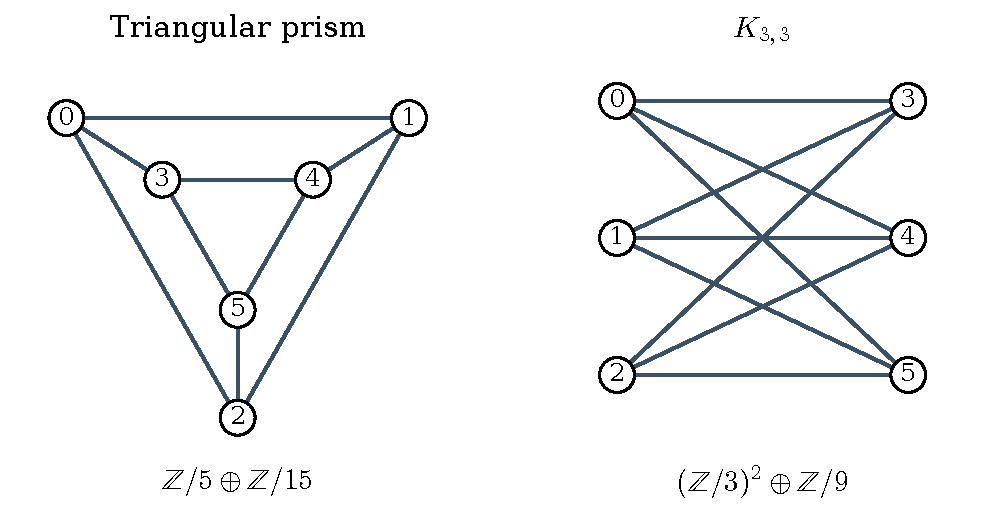
\includegraphics[width=\textwidth]{figures/output/monodromy-graphs.pdf}
 \caption{Two attachment graphs for the same six
 triply pointed rational components. The local
 component metrics and first-order node metric
 germs can be identical. The integral monodromy
 torsion groups have different orders, $75$ and $81$.
 The diagram depicts the exact attachment data;
 it is not a numerical spectral experiment.}
 \label{fig:monodromy-graphs}
\end{figure}

Both smooth fibres have genus four,
and their rational nilpotent
monodromy ranks are four.
Their smooth surfaces therefore
have the same diffeomorphism type.
What differs is an integral
invariant of the degeneration.
The local geometric inputs alone
do not determine it; the marked
global low-mode data determine
the missing adjacency and hence
the integral form.

This conclusion uses the full
Gram form for the conjugacy class;
the Smith diagonal records only
its cokernel group. Parallel
edges are excluded because sums
of their transported off-diagonal
blocks can cancel. Unknown
smoothing orders would change
the monodromy pairing to
$Z^T\operatorname{diag}(n_e)Z$
and require additional observations.
Neither the minimality of the
present observation package nor
recovery from unmarked eigenvalues
is asserted.

\section{Further questions}\label{sec:questions}

The preceding theorems distinguish three kinds of information.
The transported energy controls the complete weak linearized
spectrum. The nonlinear reconstruction also requires the
component and collar estimates for the actual Chern curvature.
Integral monodromy is obtained only after the marked observations
have determined the missing incidence and the first-order
smoothing has fixed its integral pairing. Several extensions
require additional arguments at precisely these distinctions.

\subsection{The weakest nonlinear time}
Proposition~\ref{prop:three-scales} gives a compact stable
rank-two family whose weakest eigenvalue has order $h^4$,
whereas its largest edge weight has order $h$.
Thus $L_*\asymp h^{-1}$ and $L_*\nu_0\asymp h^3$.
Theorem~\ref{thm:tracking} controls bounded intervals
of order $h^{-1}$. Its residual estimate, integrated
to order $h^{-4}$, gives a bound of order
$h^{-2}(1+|\log h|)^2$, which does not tend to zero.
The all-time hypothesis of Theorem~\ref{thm:all-time}
therefore cannot be removed by the same argument.

\begin{question}
For the family of Proposition~\ref{prop:three-scales},
does a finite nonlinear evolution track the actual
HYM flow uniformly through the time $h^{-4}$ for
the spatial initial class of Section~\ref{sec:entry}?
If so, is the leading equation
\eqref{eq:finite-flow} sufficient, or must it be
corrected?
\end{question}

Failure of the integrated upper bound is not a
counterexample to tracking. Both exact and finite
solutions can retain a weak component for a long
time. A useful proof might estimate the residual
relative to the evolving dissipation, or incorporate
the next terms in the finite field. Either approach
must retain cancellations among the incident
forces; a bound on each force separately can lose
the scale of their sum. Relative linear spectral
comparison alone does not settle this question.

\subsection{Independent nodes with component holonomy}
Section~\ref{sec:component-holonomy} permits arbitrary
ratios of the component energy to the common neck
energy. Sections~\ref{sec:geometry}--\ref{sec:entry}
permit arbitrary ratios of the six node energies
when the component connections are trivial.
Combining these results requires a compact family
with both sets of independent parameters and an
analysis on that family. In particular, the
harmonic gauges on the punctured components must
give energy-controlled boundary estimates at each
individual neck, and the nonlinear matching must
retain the component connection terms. An abstract
sum of the two proved operators would not verify
these requirements.

\subsection{Nonunitary degeneration and singular limits}
All bundles used in this paper admit flat unitary
reference connections. Their holomorphic structures
are polystable, and the degenerations of stability
studied here concern reducibility and the
appearance of parallel endomorphisms. Genuine
nonunitary extensions can introduce additional
deformation and obstruction terms into the
effective equation. Unstable holomorphic bundles
also lack the stationary reference metric used
in the order bounds and tail estimates.
Their actual HYM evolution requires a different
normalization and confinement argument.

On a smooth curve, varying the Kähler form alone
does not produce ordinary slope walls. A broader
stability problem must be realized by varying
holomorphic bundle data, a specified parabolic
stability structure, or higher-dimensional
polarizations. When singular graded sheaves or
curvature concentration occur, their local charge
and scale data must enter the matching problem.
No singular concentration law follows from the
flat-bundle results proved here.

\subsection{Conditioning and additional observations}
For a known graph with independent weights,
Theorem~\ref{thm:projective-inverse} resolves an edge
only when the observed block error is small
relative to that edge's weight. An observation
scheme adapted to successively weaker spectral
subspaces might recover smaller weights, but
would require compatible markings and a sharper
operator estimate. Eigenvalue accuracy by itself
does not provide these identifications.

For unknown incidence,
Theorem~\ref{thm:monodromy-inverse} uses a finite
simple-graph class, known first-order node
smoothing and component averages of eigenvectors.
Parallel edges, unknown smoothing multiplicities
and unmarked component permutations require
different observations. It would be useful to
identify a minimal sufficient observation package
and to quantify the propagation of errors from
raw eigenvalue and eigensection measurements.
The present operator-level error margin does not
answer that statistical or numerical question.

\subsection{Higher-dimensional geometry}
The curve construction separates component
parallel endomorphisms from the directions
coupled by the nodes. In higher dimensions
both that decomposition and the local capacity
law can change. A bundle theorem must identify
the actual endomorphism complex, construct its
compact holomorphic family, and prove the
uniform analytic estimates in the chosen
Kähler metrics. Small eigenvalues of ordinary
differential forms do not automatically give
the required endomorphism modes.
Likewise, recovering projective bundle transport
does not recover the integral cohomology of
the base. A higher-dimensional synthesis must
specify and prove each connection on the same
geometric family.

\begin{thebibliography}{HKKP18}
\bibitem[AO20]{achinger-ogus}
P.~Achinger and A.~Ogus, \emph{Monodromy and log geometry},
Tunisian J. Math. \textbf{2} (2020), no.~3, 455--534.
\href{https://doi.org/10.2140/tunis.2020.2.455}{doi:10.2140/tunis.2020.2.455}.

\bibitem[BHN97]{bacher-harpe-nagnibeda}
R.~Bacher, P.~de la Harpe and T.~Nagnibeda,
\emph{The lattice of integral flows and the lattice of integral cuts on a finite graph},
Bull. Soc. Math. France \textbf{125} (1997), no.~2, 167--198.
\href{https://doi.org/10.24033/bsmf.2303}{doi:10.24033/bsmf.2303}.

\bibitem[Bha13]{bhatia}
R.~Bhatia, \emph{The Riemannian mean of positive matrices}, in
\emph{Matrix Information Geometry}, F.~Nielsen and R.~Bhatia (eds.),
Springer, 2013, pp.~35--51.
\href{https://doi.org/10.1007/978-3-642-30232-9_2}{doi:10.1007/978-3-642-30232-9\_2}.

\bibitem[Bur90]{burger}
M.~Burger, \emph{Small eigenvalues of Riemann surfaces and graphs},
Math. Z. \textbf{205} (1990), 395--420.
\href{https://people.math.ethz.ch/~burger/pub/1990_Small_eigenvalues.pdf}{Author's published copy}.

\bibitem[DW93]{dw-local}
G.~D.~Daskalopoulos and R.~A.~Wentworth,
\emph{Local degeneration of the moduli space of vector bundles and factorization of rank two theta functions. I},
Math. Ann. \textbf{297} (1993), 417--466.
\href{https://math.umd.edu/~raw/papers/local.pdf}{Author's published copy}.

\bibitem[DW00]{dw}
G.~D.~Daskalopoulos and R.~A.~Wentworth,
\emph{The Yang--Mills flow near the boundary of Teichm\"uller space},
Math. Ann. \textbf{318} (2000), no.~1, 1--42.
\href{https://doi.org/10.1007/s002080000098}{doi:10.1007/s002080000098}.

\bibitem[DM69]{deligne-mumford}
P.~Deligne and D.~Mumford,
\emph{The irreducibility of the space of curves of given genus},
Publ. Math. Inst. Hautes Études Sci. \textbf{36} (1969), 75--109.
\href{https://doi.org/10.1007/BF02684599}{doi:10.1007/BF02684599}.

\bibitem[Don85]{donaldson}
S.~K.~Donaldson,
\emph{Anti self-dual Yang--Mills connections over complex algebraic surfaces and stable vector bundles},
Proc. London Math. Soc. (3) \textbf{50} (1985), no.~1, 1--26.
\href{https://doi.org/10.1112/plms/s3-50.1.1}{doi:10.1112/plms/s3-50.1.1}.

\bibitem[Flo01]{florentino}
C.~Florentino,
\emph{Schottky uniformization and vector bundles over Riemann surfaces},
Manuscripta Math. \textbf{105} (2001), no.~1, 69--83.
\href{https://doi.org/10.1007/PL00005874}{doi:10.1007/PL00005874}.

\bibitem[Gol84]{goldman}
W.~M.~Goldman,
\emph{The symplectic nature of fundamental groups of surfaces},
Adv. Math. \textbf{54} (1984), 200--225.
\href{https://doi.org/10.1016/0001-8708(84)90040-9}{doi:10.1016/0001-8708(84)90040-9}.

\bibitem[Gra60]{grauert}
H.~Grauert,
\emph{Ein Theorem der analytischen Garbentheorie und die Modulräume komplexer Strukturen},
Publ. Math. Inst. Hautes Études Sci. \textbf{5} (1960), 5--64;
correction, \textbf{16} (1963), 35--36.
\href{https://doi.org/10.1007/BF02684746}{doi:10.1007/BF02684746}.

\bibitem[HKKP18]{hkkp}
F.~Haiden, L.~Katzarkov, M.~Kontsevich and P.~Pandit,
\emph{Iterated logarithms and gradient flows}, preprint, 2018.
\href{https://arxiv.org/abs/1802.04123v1}{arXiv:1802.04123v1}.

\bibitem[HK14]{hubbard-koch}
J.~H.~Hubbard and S.~Koch,
\emph{An analytic construction of the Deligne--Mumford compactification of the moduli space of curves},
J. Differential Geom. \textbf{98} (2014), no.~2, 261--313.
\href{https://doi.org/10.4310/jdg/1406552251}{doi:10.4310/jdg/1406552251}.
\href{https://arxiv.org/abs/1301.0062v1}{arXiv:1301.0062v1}.

\bibitem[Lam26]{lam}
S.~T.~Lam, \emph{Semistability and asymptotics of geometric flows},
preprint, 2026.
\href{https://arxiv.org/abs/2606.09235v1}{arXiv:2606.09235v1}.

\bibitem[NS65]{narasimhan-seshadri}
M.~S.~Narasimhan and C.~S.~Seshadri,
\emph{Stable and unitary vector bundles on a compact Riemann surface},
Ann. of Math. (2) \textbf{82} (1965), no.~3, 540--567.
\href{https://doi.org/10.2307/1970710}{doi:10.2307/1970710}.

\bibitem[Wue26]{wuebben-hym}
B.~J.~Wuebben, \emph{Effective Hermitian--Yang--Mills flow on nodal degenerations of curves},
preprint, 10 November 2026.
\href{https://doi.org/10.5281/zenodo.24120966}{doi:10.5281/zenodo.24120966}.
\end{thebibliography}

\end{document}
